
\documentclass[draft,linenumbers]{agujournal}
\draftfalse
\journalname{Journal of Advances in Modeling Earth Systems (JAMES)}
\begin{document}


\title{Implementing plant hydraulics in the Community Land Model}
\authors{Daniel Kennedy\affil{1},
Sean Swenson\affil{2},
Keith Oleson\affil{2},
David Lawrence\affil{2},
Rosie Fisher\affil{2},
Pierre Gentine\affil{1}
}


\affiliation{1}{Columbia}
\affiliation{2}{NCAR}
\correspondingauthor{Daniel Kennedy}{djk2120@columbia.edu}

\begin{keypoints}
\item A simplified soil-plant-atmosphere continuum model is implemented in CLM5
\item Prognostic leaf water potential replaces soil matric potential as the functional basis for water stress, reflecting xylem tension constraints and vegetation sensitivity to atmosphere drying. 
\item Prognostic root water potential is used to implement hydraulic root water uptake, replacing a soil wilting factor heuristic.
\end{keypoints}



\begin{abstract}
= enter abstract here =
\end{abstract}

%====================
%  INTRODUCTION
%====================

\section{Introduction}

Trees face emerging climate change risk globally \citep{allen2010,anderegg2013b}.
Understanding vegetation response is a high priority, both for discerning climate impacts and for modeling feedbacks to the carbon and hydrological cycles.
While there are disagreements about soil moisture trends globally \citep{dai2013,sheffield2012}, 
Amazonia has experienced and a lengthening dry season \citep{fu2013} and faces projections of increasing frequency of extreme El Ni\~no events \citep{cai2014}.
In addition to stress from soil moisture drought, vegetation are susceptible to increasing atmospheric transpiration demand \citep{restaino2016,novick2016b}.
Increases in vapor pressure deficit (VPD) have occurred with warming \citep{ficklin2017,seager2015}, and are associated with impacts on vegetation \citep{williams2013,mcdowell2015}.
However, significant uncertainty remains regarding how vegetation will respond to changes in hydroclimate within Earth System Models \citep{dekauwe2017,friedlingstein2014}.
In this study, we update the CLM water stress parameterization based on hydraulic theory and
analyze its dynamics with a set of point simulations set within the Caxiuan\~a throughfall exclusion experiment \citep{fisher2006}.

Plant hydrodynamic parameterizations are important in Earth System Models, defining vegetation regulation of latent heat flux.
Vegetation water use strategies also modulate carbon uptake, creating a critical coupling between the Earth System's carbon and hydrological cycles.
Typically drought stress parameterizations are used to define a notion of vegetation water status 
that is used to attenuate transpiration, photosynthesis, and root water uptake with drying.
The dynamics of water stress in models have broad effects on critical land surface process.
On diurnal timescales drought parameterizations influence partitioning of latent versus sensible heat with effects on surface temperature \citep{bonan2014}.
On longer timescales vegetation water use strategies regulate the global carbon and water cycles \citep{dekauwe2015}.
Representation of vegetation water stress in CLM and other models is a known deficiency, with implications for the representation of the dry/wet season in tropical rainforests \citep{powell2013,ukkola2016}.

Many recent studies have worked to advance the representation of water flow through the Soil-Plant-Atmosphere continuum (SPAC) in models \citep{xu2016,christoffersen2016,sperry2017}.
Modeling water flow through the SPAC adds complexity, but is in line with evidence of dynamic regulation of vegetation water use in response to both soil and atmospheric drying \citep{sperry2015}.
Furthermore, via Darcy's Law, SPAC models have a robust physical basis.
Parameter estimation is challenging \citep{drake2017}, but hydraulic trait information is available \citep{kattge2011,anderegg2015a} and can be informative of forest vulnerability to drought \citep{choat2012}.
Likewise vegetation water status observations are available at a scale that is directly relevant to model development \citep{konings2016,grant2016} and can be used to validate model results \citep{momen2017,konings2017b}.

Advancing the representation of the SPAC introduces a new state variable to CLM, vegetation water potential, 
which is valuable for modeling both vegetation water supply and transpiration demand.
Modeling vegetation water potential, allows for a physical representation of water supply, from the soil through the vegetation substrate.
This can incorporate a range of water use strategies, and improves the model connection between allocation decisions and water availability.
Likewise, root water uptake can be based on Darcy's law, in lieu of an empirical transpiration partitioning heuristic.
Modeling vegetation water potential also creates a framework for representing hydraulic redistribution \citep{lee2005}.
Water demand is typically attenuated with drought stress, according to vegetation water status, capturing dynamic vegetation water use regulation.
Leaf water potential serves as an improved metric for water status, in lieu of soil water or soil matric potential.
This reflects vegetation sensitivity to both soil and atmospheric drying, while serving as a diagnostic for excessive xylem tension and cavitation risk.

This provides a basis for the objectives of this study.
We developed a simplified plant hydraulic implementation within CLM5, Plant Hydraulic Stress (PHS).
This sets a framework to represent vegetation water potential, which is used to improve model vegetation hydrodynamics.
Leaf water potential replaces soil potential, as the functional basis for drought stress attenuation of transpiration and photosynthesis.
Root water potential is used to model gradient-based root water uptake in lieu of a soil wilting factor heuristic.
To assess the new model formulation, we carried out point simulations at Caxiuan\~a National Forest in Brazil.
This site features a critical biome subject to experimental throughfall exclusion, where we expect vegetation regulation of turbulent fluxes.
We compare PHS with the former CLM hydrodynamics model, analyzing the dynamics of modeled water stress and root water uptake.

%====================
%  MODEL DESCRIPTION
%====================
\section{Model Description}

%Photosynthesis
\subsection{Photosynthesis}
\label{sect:A}
    The CLM5 photosynthesis model is largely inherited from CLM4.5 as described in \citet{bonan2011}, \citet{thornton2007},
    and \citet{oleson2013}.Photosynthesis is defined in three regimes: Rubisco-limited, light-limited, and export-limited 
    following \citet{farquhar1980} and \citet{harley1992}.The implementation extends \citet{sellers1996a,sellers1996b} with 
    colimitation following \citet{collatz1991}. 
    
    CLM5 photosynthesis, in its default configuration, is a two-big-leaf model, with a sunlit and shaded leaf for each plant functional type \citep{thornton2007, dai2004, oleson2013}. 
    The canopy fluxes module iterates for leaf surface energy balance.
    Within this, the photosynthesis module iterates to solve for intercellular CO$_2$ concentration, balancing stomatal flux of 
    CO2 with photosynthetic assimilation flux of CO2.
    
    Vegetation water stress is implemented via the vegetation water stress factor ($f_w$, dimensionless, 0 to 1, formerly $\beta_t$). 
    There are many different approaches for how to apply stress \citep{zhou2013,novick2016a,sperry2015}.
    In CLM, $f_w$ multiplies the rate of maximum carboxylation ($V_{\text{cmax}}$) as described in \citet{oleson2013}.
    While many models opt for soil-moisture based stomatal limitation (linking the stomatal conductance model slope parameter to soil moisture),
    \cite{lin2018} found that only $g_0$ was sensitive to soil moisture (and not $g_1$).
    \cite{zhou2013} suggests that changes in assimilation tend to exceed those predicted by modulating $g_1$ with soil moisture, but could be captured by changing $V_{\text{cmax}}$.
    Some field studies suggest $V_{\text{cmax}}$ is not changing with drought, whereby model $V_{\text{cmax}}$ instead may implicitly account for mesophyll conductance changes \citep{flexas2004}.
    
    With PHS, $f_w$ replaces the CLM4.5 transpiration beta function ($\beta_t$). 
    These factors are used by the photosynthesis model in the same way, but calculated differently. 
    The PHS parameterization for $f_w$ is based on leaf water potential (see Section \ref{sect:demand}) . 
    Previously the parameterization was based on soil water potential (see Section \ref{sect:btran}).
    Utilizing leaf water potential adopts a framework where stomatal conductance optimized for carbon gain is concurrently limited by hydraulic constraints \citep{novick2016a}.


%Stomatal Conductance
\subsection{Stomatal Conductance}
\label{sect:gs}
    CLM5 uses the Medlyn stomatal conductance model, which reconciles the empirical and optimal approaches to modeling 
    stomatal conductance \citep{medlyn2011}. 
    Stomatal conductance of CO2 is related to net photosynthesis ($A_n$), CO2 concentration at the leaf surface 
    ($C_a$), and the square root of the vapor pressure deficit near the leaf surface ($\sqrt{D}$).
    \begin{equation}
    g_s=g_0+\left(1+\dfrac{g_1}{\sqrt{D}}\right)\dfrac{A}{C_a}
    \end{equation}
    The model features two parameters $g_0$ ($\mu$mol / m2 / s) and $g_1$ (kPa$^{0.5}$). 
    The $g_0$ parameter is minimum stomatal conductance, representing cuticular and epidermal losses (small). 
    The $g_1$ parameter relates to the marginal water cost guiding the optimization of carbon assimilation.
    
    The Medlyn model, derived from stomatal optimization theory, predicts stomatal conductance to maximize assimilation relative to water costs ($A-\lambda E$), 
    but does not resolve concurrent limitations to stomatal conductance associated with drought conditions.
    Much recent work has focused on concurrent limitations on plant hydrodynamics, especially in response to drying soils \citep{manzoni2013b,novick2016a,zhou2014}.
    For example, plants must also manage the risk of cavitation associated with increasing xylem tension \citep{sperry1998}.
    Stomatal representation within land surface models typically include a drought stress factor, with various approaches for where to apply stress.
    
    Drought stress factors (in our case, $f_w$), are used to model stomatal and non-stomatal limitation associated with water stress.
    Uncertainty remains within the literature for how to apply water stress to photosynthesis and stomatal conductance.
    One line of reasoning eschews the optimization of $A-\lambda E$ in favor of hydraulic costs \citep{sperry2017},
    Studies also explore soil water adjustments to the marginal water cost, implemented by adjusting $\lambda$ or Medlyn's $g1$ based on soil water \citep{manzoni2013b}.
    However, this may underestimate drought effects on photosynthesis \citep{zhou2013,lin2018}.
    Yet other groups take a hybrid approach, combining optimal stomatal conductance, with hydraulic constraints and/or
    so-called non-stomatal limitation, attenuating $V_{\text{cmax}}$ or mesophyll conductance
    (which feeds back through photosynthesis to lower stomatal conductance) \citep{egea2011,novick2016a}.
    
    We opt for a simplified form of this last approach, which seems to be consistent with field observations \citep{lin2018}.
    For PHS, the attenuation of stomatal conductance due to water stress follows the CLM4.5 formulation as described in \citet{oleson2013} and \citet{bonan2011}. 
    Prognostic water stress ($f_w$, ranging from 0-1) attenuates stomatal conductance indirectly via multiplication of $V_{\text{cmax}}$.
    Water stress lowers assimilation, which is coupled to stomatal conductance.
    
% Plant Hydaulics
\subsection{Plant Hydraulic Stress (PHS)}
  In this study, we implemented a simplified plant hydraulic framework into CLM5 to calculate root water uptake and water stress attenuation of photosynthesis and transpiration.
  Using hydraulic laws and the corresponding circuit analogy, we model the flow of water through the soil-plant-atmosphere continuum. 
  The hydraulic framework is used to diagnose water stress associated with increasing xylem tension
  and to calculate the root water uptake in each of (in this case) 20 vertically discretized soil layers.
  The combined water supply and demand implementations governing vegetation hydrodynamics is called Plant Hydraulic Stress (PHS).
  On the demand side, PHS redefines $f_w$, the CLM water stress factor, utilizing leaf water potential as its indicator for plant water status in lieu of soil potential.
  On the supply side, PHS adopts Darcy's Law to model root water uptake, replacing a soil-wilting-factor heuristic.
  By modeling vegetation water potential, we advance the physical basis plant water use, 
  improving the dynamics of turbulent fluxes and root water uptake in response to water stress. 

  \begin{figure}[h]
     \centering
     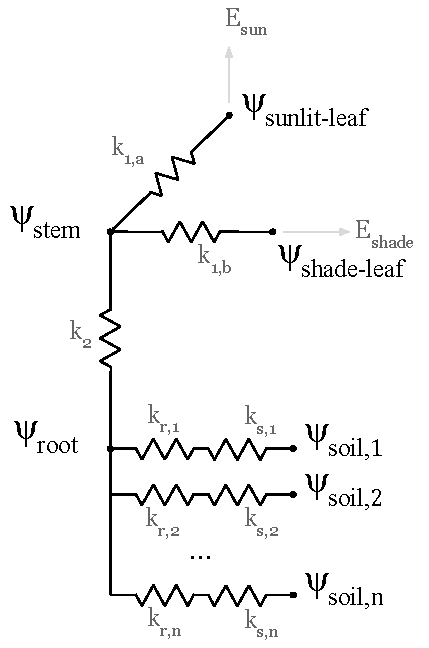
\includegraphics[width=9pc]{../figs/circuit.pdf}
     \caption{Plant hydraulic circuit analog schematic}
     \label{circuit}
  \end{figure}

%Hydraulic schematic and segmentation
  \subsubsection{Hydraulic schematic and segmentation}
  PHS solves for the set of vegetation water potential values 
  ($\psi_{\text{root}}$, $\psi_{\text{stem}}$, $\psi_{\text{shade-leaf}}$, $\psi_{\text{sun-leaf}}$ ) 
  that matches water supply (root water uptake) to water demand (transpiration), 
  while maintaining continuity of water flow throughout the soil-plant-atmosphere continuum.
  The PHS circuit analogy is presented in Figure \ref{circuit}.
   Segmentation and other model design decisions followed a preference for a simplified implementation that,
  whenever possible, conformed to existing CLM model structure.
  
  At each node in the circuit diagram, we model water potential, and, between nodes, we resolve the flux of water.
  The segmentation is designed to take advantage of field-measured hydraulic traits and to allow for differences
  in segment parameterizations \citep{simonin2015, sperry2015}.
  Following from CLM, we utilize vertically discretized soil layers and a two-layer (sunlit vs. shaded) canopy.
  Soil layers are assumed to operate in parallel, which is a typical assumption justified by higher resistance in lateral versus central roots.
  Based on Darcy's law, we additionally segment the resistance across the soil matrix from the resistance through the root tissue \citep{williams1996}. 
  Specifics on the parameterization of conductance for each segment are provided in Appendix B.1.

%Water Supply
    \subsubsection{Water supply}
    \label{sect:supply}
    Water supply is modeled via Darcy's Law, where flow is proportional to the gradient in water potential. 
    Flow of water ($q$) is the product of the path hydraulic conductance ($k$) and 
    the gradient in water potential (accounting for changes in gravitational potential). 
    Equation \ref{eq:darcy} represents the flow from a generic node 1 to node 2. 
    
     \begin{linenomath*}
     \begin{equation}
     \label{eq:darcy}
     q = -k\left(\psi_2 - \psi_1 - \rho g \Delta z\right)
     \end{equation}
     \end{linenomath*}
    
    PHS does not represent plant tissue water storage (by circuit analogy: capacitance). 
    Capacitance significantly complicates the water potential solution \citep{celia1990} and is challenging to parameterize \citep{bartlett2016}.   
     However, buffering of water stress provided by tissue water storage could potentially be important especially on sub-daily timescales \citep{meinzer2009,epila2017}, whereby its inclusion may be warranted in future model generations.

     Vegetation segment conductance is modeled following empirical xylem vulnerability curves \citep{tyree1989}, 
     where segments lose conductance with increasing xylem tension related to 
     cavitation and embolism \citep{holbrook2001}.
     The vulnerability curves model loss of conductance relative to maximum conductance using two parameters: 
     $c_k$, a sigmoidal shape-fitting parameter, and 
     $p_{50}$, the water potential at 50\% loss of segment conductance (following \cite{gentine2016}). 
     These parameters can be estimated from field experiments \citep{sack2002}, 
     and $p_{50}$ is available in the TRY trait database \citep{kattge2011}.
     Parameterization based on $p_{50}$ aligns with the call for a transition to a
     trait-based model paradigm \citep{anderegg2015a}.
     The loss of xylem conductivity is based on lower terminus water potential ($\psi_1$)
     as is typical in other simplified models \citep{xu2016}, but 
     may underestimate the integrated loss of conductivity \citep{sperry2015}. 
         
     \begin{linenomath*}
     \begin{equation}
     \label{eq:vulnerability}
     k = k_{\text{max}} \, 2^{-\left(\dfrac{\psi_1}{p_{50}}\right)^{c_k}}
     \end{equation}
     \end{linenomath*}
     
     PHS models root, stem, and leaf tissue conductances according to equation \ref{eq:vulnerability}.
     The parameterization of $k_{\text{max}}$ varies by hydraulic segment (see details in Appendix B1).
     The conductance across the soil matrix to the root surface follows \citet{williams2001} and \citet{bonan2014} 
     to estimate a characteristic distance between roots for the length-scaling of soil conductivity.
     Bulk soil resistivity is based on \citet{clapp1978} as described in \citet{oleson2013}.
     Further details are provided in Appendix B1.
    
%Water demand
    \subsubsection{Water demand}
    \label{sect:demand}
    
    Vegetation water demand and stomatal regulation is based on the Medlyn stomatal conductance model (see Section \ref{sect:gs}), 
    which we adjust for water stress with $f_w$, the CLM water stress factor. 
    The water stress factor multiplies $V_{\text{cmax}}$, which indirectly attenuates stomatal conductance.
    We calculate the water stress factor based on leaf water potential, which has been shown to correspond to stomatal sensitivity \citep{klein2014}.
    This is an update to CLM4.5, which bases $f_w$ on soil water potential \citep{oleson2013}.
    However, once calculated, $f_w$ is deployed in the same way across versions of CLM (multiplies $V_{\text{cmax}}$).

     \begin{linenomath*}
     \begin{eqnarray}
     \begin{aligned}
     \label{eq:demand}
     E_{\text{sun}}     &= E_{\text{sun,max}} \, 2^{-\left(\dfrac{\psi_{\text{sun-leaf}}}{\psi_{50}}\right)^{c_k}} \\
     E_{\text{shade}} &= E_{\text{shade,max}} \, 2^{-\left(\dfrac{\psi_{\text{shade-leaf}}}{\psi_{50}}\right)^{c_k}}
     \end{aligned}
     \end{eqnarray}
     \end{linenomath*}
    
    
     \begin{linenomath*}
     \begin{eqnarray}
     \begin{aligned}
     \label{eq:stress}
     f_{\text{w,sun}}         &= \dfrac{g_{\text{s,sun}}}{g_{\text{s,sun,max}}} \\
     f_{\text{w,shade}}     &= \dfrac{g_{\text{s,shade}}}{g_{\text{s,shade,max}}} \\
     \end{aligned}
     \end{eqnarray}
     \end{linenomath*}
    
     As leaf water potential declines and xylem tension increases, transpiration is attenuated relative to maximal values.
     The maximum transpiration ($E_{\text{sun,max}}$, $E_{\text{shade,max}}$) is that resulting from Medlyn stomatal conductance absent water stress (achieved by setting $f_w=1$)
     The fraction of maximum transpiration is modeled with a two-parameter sigmoidal function (Equation \ref{eq:demand}). 
     The parameters are $\psi_{50}$, the leaf water potential at 50\% loss of transpiration and 
     $c_k$ a sigmoidal shape-fitting parameter.
    
    The value of $f_w$ is based on the solution for attenuated transpiration.
    We define $f_w$ as the ratio of attenuated to maximal stomatal conductance (Equation \ref{eq:stress}).
    Maximum stomatal conductance ($g_{\text{s,sun,max}}$, $g_{\text{s,shade,max}}$) is the stomatal conductance when calculated with $f_w=1$
    (i.e. without water stress). 
    The attenuated stomatal conductance ($g_{\text{s,sun}}$, $g_{\text{s,shade}}$) is the stomatal conductance associated with the PHS module
    water flow solution, which matches vegetation water supply with vegetation water demand 
    (Section \ref{sect:solution}).
    
     Whereas the water supply parameters (see Section \ref{sect:supply}) relate to hydraulic traits often measured in the field, 
     the hydraulic demand parameters $\psi_{50}$ and $c_k$ reflect the emergent property of hydraulic limitations to transpiration and must be empirically derived. 
     Likewise CLM4.5 had two empirical stomatal control parameters, which were the soil matric potentials 
     corresponding to stomates fully closed and stomates fully open (see Section \ref{sect:btran}).
     The functional form of stomatal control is not generally agreed upon, and as such, should be investigated further. 
     Recent modeling studies have proposded differnt forms sperry,xu,christo. 
     However observations (lin et al. 2018) seem to suggest that $psi_l$ mainly affects the GPP compeonent of gs and thus Vc,max and not the other comeopnents (g1 and g0 in the Medlyn paramterization).

%PHS solution
    \subsubsection{PHS solution}
    \label{sect:solution}
    
    PHS solves for the set of vegetation water potential values ($\psi$) that matches water supply
    (root water uptake) to water demand (transpiration), while satisfying continuity across the four water flow
    segments (soil-to-root, root-to-stem, stem-to-leaf, and leaves-to-transpiration). 
    We compute the flux divergence $f$ (representing the mismatch of flow in and out of each segment)
    for a given set of vegetation water potential values $\psi_i$, and iteratively update $\psi$ until $f\to0$.
    
    \begin{linenomath*}
    \begin{equation} 
    \psi = \left[
    \begin{array}{c}
    \psi_{\text{sun}} \\ 
    \psi_{\text{shade}} \\ 
    \psi_{\text{stem}} \\ 
    \psi_{\text{root}}            
    \end{array} \right]
    \end{equation}
    \end{linenomath*}
    
    \begin{linenomath*}
    \begin{equation}
    f\left(\psi\right) = \left[ 
    \begin{array}{c}
    E_{sun}-q_{sun}\\
    E_{shade}-q_{shade}\\
    q_{sun}+q_{shade}-q_{stem}\\
    q_{stem}-\sum_{j=1}^n{q_{root,j}}
    \end{array} \right]
    \end{equation}
    \end{linenomath*}
    
    \begin{linenomath*}
    \begin{equation}
    A = \dfrac{df}{d\psi}
    \end{equation}
    \end{linenomath*}    
    
    While $\left|f\right|>0$
    \begin{linenomath*}
    \begin{equation} \begin{aligned}
    \label{eq:iter}
    \Delta\psi &=A^{-1}f\left(\psi_i\right) \\
    \psi_{i+1}  &= \psi_i + \Delta\psi
    \end{aligned} \end{equation}
    \end{linenomath*}    
    
    The numerics are especially tractable because $f$ has analytical derivatives and $A$ 
    (a 4x4 matrix with six null entries) is easy to invert when well-conditioned. 
    Supply and demand converge, because transpiration demand decreases with more negative 
    leaf water potentials and supply increases with more negative leaf water potentials.
    Within a set of PHS iterations (\ref{eq:iter}), transpiration is assumed to be linear with $f_w$.
    PHS is nested within iterations for intercellular CO$_2$ concentration and leaf temperature.
    The non-linear relationship between $f_w$ and transpiration is resolved through iteration for converging $f_w$ alongside intercellular CO$_2$.
    Details on the numerical implementation are provided in Appendix Section B.1.

%====================
%  BTRAN
%====================

\section{Water stress factor, SMS vs. PHS}
\label{sect:btran}
    PHS alters the transpiration beta function ($\beta_t$, colloquially BTRAN), 
    which is the phenomenological soil water stress function in CLM2-CLM4.5, as described in \citet{oleson2013}.
    Because the name $\beta_t$ is associated with this specific plant hydrodynamics representation, we opt to rename the variable to $f_w$ (water stress factor).
    Throughout this paper we refer to the CLM4.5 plant hydrodynamics framework as SMS (soil moisture stress), 
    as compared to the newer implementation, PHS (plant hydraulic stress).
    We adopt this terminology (in lieu of CLM4.5 vs. CLM5), because SMS is still deployable with CLM5. 
    
    With PHS, we interpret $f_w$ as a drought safety mechanism, attenuating stomatal conductance to avoid
    excessive xylem tension associated with very negative leaf water potential.
    As such, $f_w$ is parameterized as a function of prognostic leaf water potential.
    With SMS, $f_w$ is calculated based on soil matric potential, 
    as a root-fraction weighted average of an empirical soil layer wilting factor (Equation \ref{bt:1}).
    In both parameterizations, $f_w$ multiplies $V_{\text{cmax}}$, attenuating photosynthesis and transpiration with drought.
    Recent studies suggest that the SMS parameterization introduces model bias in turbulent fluxes \citep{bonan2014}
    and contributes to unrealistic drought response of photosynthesis and stomatal conductance \citep{powell2013}.

    
    Such parameterizations have primarily been examined with application to stomatal conductance, but they are also used to define vegetation soil water extraction. 
    Each timestep, the transpiration flux solution must be distributed among the vertically discretized soil layers.
    In the SMS framework, the transpiration sink is partitioned by layer according to the soil layer wilting factor and root fraction.
    This framework lacks several key physical attributes of soil water extraction, which are addressed in the PHS implementation.
    In this section we present the SMS version of $f_w$ and outline the differences as compared to PHS.
    
    The variable $f_w$ is unitless, ranging from 0 to 1, with 1 corresponding to no water stress, and 0 corresponding to fully water stressed. 
    It is calculated based on a root-fraction weighted average of soil layer wilting factor ($w_i$), which is a bounded linear 
    function of soil water potential ($\psi_i$) relative to PFT parameters defining the soil potential with stomates fully open ($
    \psi_{o}$) and fully closed ($\psi_{c}$), among the soil layers $i=1,...\,,n$. Note that root fraction ($r_i$) sums to 1, by definition.
    
    \begin{linenomath*}
    \begin{equation} f_w = \sum_{i=1}^{n}{r_iw_i}
    \label{bt:1}
    \end{equation}
    \begin{equation} 
    \label{bt:2}
    w_i=0 \leq \dfrac{\psi_i-\psi_{c}}{\psi_{o}-\psi_{c}} \leq 1
    \end{equation}
    \end{linenomath*}
    
    In both stress parameterizations, $f_w$ multiplies $V_{\text{cmax}}$ to attenuate photosynthesis and stomatal conductance with soil water stress. 
    With SMS, it is also directly used for modeling vegetation water extraction from the soil column. 
    The total transpiration ($T$) is partitioned among the soil layers based on the $f_w$ wilting factor. 
    Within each soil layer, the flux to transpiration ($q_i$) depends on the layer root fraction and wilting factor, normalized by $f_w$.

    \begin{linenomath*}
    \begin{equation}
    \label{bt:4}
    q_i = \dfrac{r_i w_i}{f_w}T
    \end{equation}
    \end{linenomath*}
    
    The PHS implementation adopts a hydraulic framework, where the root water uptake ($q_i$) is 
    the product of the hydraulic conductance ($k_i$) and the gradient in water potential (-$\Delta\psi$) driving the flow.
    That gradient is the difference between the root water potential ($\psi_{\text{root}}$) and the layer soil water potential ($\psi_i$), less changes in gravitational potential.
    \begin{linenomath*}
    \begin{equation}
        \begin{aligned}
    q_i &= -k_i \Delta\psi \\
    \Delta\psi &= \left(\psi_{\text{root}}-\psi_{i}-\rho g \Delta z\right)
    \label{phs:sink}
    \end{aligned}
    \end{equation}
    \end{linenomath*}
    
    For comparison, we recast (\ref{bt:4}) into the hydraulic framework: defining $T_{\text{max}}$, such that: $T = 
    f_w T_{\text{max}}$ to replace $T$ in (\ref{bt:4}), and replacing $w_i$ in (\ref{bt:4}) with the formula from (\ref{bt:2}).
    
    \begin{linenomath*}
    \begin{equation} 
    q_i = \dfrac{T_{\text{max}}}{\psi_{o}-\psi_{c}} r_i \left(\psi_i-\psi_{c} \right)
    \end{equation}
    \end{linenomath*}
    
    This yields SMS analogs for the hydraulic conductance and gradient terms of Equation \ref{phs:sink}.
    \begin{linenomath*}
    \begin{equation} \begin{aligned}
    k_i &= r_i \, \dfrac{T_{max}}{\psi_{o}-\psi_{c}} \\
    \Delta\psi &=  \psi_{c}-\psi_i \\
    \mbox{constrained by:} \qquad
    \Delta\psi &=
    \begin{cases}
    0                          & \text{if } \psi_i<\psi_{c}  \\
    \psi_{c}-\psi_{o} & \text{if } \psi_i>\psi_{o}
    \label{kb}
    \end{cases}
    \end{aligned}\end{equation}
    \end{linenomath*}

    Here we discuss some of the unphysical implications for root water uptake from the former parameterization of water stress (Equation 15).
    
    \subsection{Constant pulling potential}
    Darcy's Law governs the flow of water through the soil-plant-atmosphere continuum, 
    with fluxes proportional to the gradient in water potential. 
    With SMS, that gradient is defined for each soil layer as 
    the difference between the soil water potential in that layer ($\psi_i$) 
    and a constant parameter, the soil water potential when stomata are fully closed ($\psi_{c}$).
    This parameter serves as the vegetation ``pulling'' potential for calculating the soil transpiration sink.
    Using a constant wilting point is inconsistent with extensive evidence from the field of dynamic vegetation water potential, and cohesion tension theory driving the transpiration flow.
    Likewise the values for $\psi_{c}$ are quite negative, (-2.5 MPa for broadleaf evergreen tropical, BET, forests). 
    \cite{fisher2006} measured midday stem potential consistently higher than -0.5 MPa during the wet season, and on average -1.69 and -1.53 MPa during the dry season in the control and exclusion plots, respectively.
    
    \subsection{Conductance dynamics}
    In lieu of dynamic vegetation water potential, intra-day SMS soil sink dynamics derive from a highly variable conductance.
    As inferred in Equation \ref{kb}, SMS conductance is modeled as a function of $T_{max}$, and three constant parameters.
    $T_{max}$ is highly dynamic, responding to the diurnal course in transpiration demand.
    This is inconsistent with general principles of porous media flow, where conductivity is a function of the hydraulic architecture and its wetted status.
    Likewise, this representation of conductance does not represent the characteristic phenomenon where vessels lose conductance with drying.
      
    \subsection{No dependence on absolute root biomass}
    As is typical, the SMS conductance is scaled by layer using an area basis.
    In this case the relative root fraction is used.
    With PHS, an absolute measure of root biomass is used (see Appendix Equation \ref{eq:rai}), so that the belowground water cycle interacts with carbon allocation to the roots.
    An absolute measure better conforms with the physics of porous media flow and better responds to varying carbon allocation strategies.
    For example, with SMS, if root mass doubles in every soil layer, the root access to water remains unchanged.

    \subsection{Lacks penalties for extraction from depth}
    Both PHS and SMS account for the effect of decreasing root area with depth (PHS, root area; SMS, root fraction), but
    PHS implements two other penalties for extracting water from deep in the soil column that are missing from SMS.
    The first is minor, but water extracted from depth must overcome gravity, amounting to about 0.01 MPa per meter in depth. 
    This is missing from SMS and included with PHS. 
    Likewise SMS ignores that hydraulic conductance is generally taken to scale with the inverse of conducting length.
    Deeper roots feature longer root tissue conducting length, and root spacing within the soil is less dense, requiring longer conducting distances across the soil matrix.
    In PHS, both these processes result in diminished hydraulic conductance.

    \subsection{Constraints}
    With SMS, the gradient in water potential is constrained between 0 and 
    the range of soil potential between parameters for stomata fully open and closed (Equation \ref{kb}). 
    The upper constraint caps the gradient in water potential when soil potential reaches the value for stomata fully open ($\psi_o$=-0.65 MPa for BET).
    Darcy's Law predicts that the gradient in water potential would continue to increase until saturation matric potential.
    The lower constraint caps the gradient in water potential at zero, disallowing negative gradients.
    However, reversed water fluxes, caused by positive gradients in water potential from root to soil, have been observed in the field \citep{burgess1998}.
    Both constraints are eschewed with PHS.     

%====================
%  EXP DESCRIPTION
%====================
\section{Experiment Description}
All four simulations in this paper use the same development version of CLM5
(development version r270, https://github.com/ESCOMP/ctsm/releases/tag/clm4
\textunderscore 5\textunderscore 18\textunderscore r270).
The four simulations are used to vary the plant hydrodynamics model (PHS vs. SMS) and throughfall forcing (Ambient vs. 60\% throughfall excluded), with all other model components and forcing shared.
Simulations are run offline, spanning from 2001 through 2003, utilizing the satellite phenology mode of CLM5.
All simulations start from the same initial conditions, which are the results of a 9-year spin-up repeating the PHS/Ambient simulation three times.
To avoid duplication, descriptions of site characteristics, forcing data, and observational sap flux, can be found in \cite{fisher2007}.

\subsection{Parameter Values and Throughfall Exclusion}
\label{sect:param}
\begin{table}
\caption{Select parameter values}
\centering
\begin{tabular}{c c c c}
CLM name & Full Name & Symbol &  Value \\
\hline
kmax(1) & Maximum Sun Branch Conductance & $k_{1a,\text{max}}$ &  4e-7 s$^{-1}$ \\
kmax(2) & Maximum Shade Branch Conductance & $k_{1b,\text{max}}$ &  4e-7 s$^{-1}$ \\
kmax(3) & Maximum Stem Conductivity & $k_{2,\text{max}}$ &  4e-7 m/s \\
krmax & Maximum Root Conductivity & $k_{r,\text{max}}$ &  6.3e-9 m/s \\
psi50 & Water potential at 50\% loss of conductivity & $\psi_{50}$ &  -2.45 MPa \\
ck & Vulnerability shape parameter & $c_k$ &  3.95 \\
smpso & Soil potential with stomata fully open & $\psi_o$ & -0.647 MPa \\
smpsc & Soil potential with stomata fully closed & $\psi_c$ & -2.5 MPa \\
medlyn\textunderscore intercept & Medlyn intercept & $g_0$ &  100 $\mu$mol / m2 / s \\
medlyn\textunderscore slope & Medlyn slope & $g_1$ &  7 kPa$^{0.5}$ \\
n & Soil porosity & $n$ & 0.42 \\
hksat & Saturated soil hydraulic conductivity & $k_{\text{s,max}}$ & 1.5e-5 m/s \\
sucsat & Saturated soil matric potential & $\psi_{\text{sat}}$ & 461 Pa \\
bsw & Brooks-Corey parameter & $b$ & 6 \\
\hline
\multicolumn{2}{l}{$^{a}$Table note text here.}
\end{tabular}
\end{table}

Select parameter values concerning vegetation hydrodynamics are presented in Table 1.
All other parameters use the default values associated with the r270 version of CLM5.
Informed by \cite{fisher2008}, we tuned soil hydraulic parameters and throughfall exclusion to better capture observational soil water dynamics (\cite{fisher2007} Figure 4), with our results shown in Supplementary Figure \ref{top3m}.
Likewise, we tuned $k_{max}$ and $g_1$ parameters to improve the fit to sap flux observations in the ambient simulation.
The object of this paper is to present the dynamics of this model instance in depth, to clearly describe model functionality without specific comment on model skill.
Model skill and parameter sensitivity will be assessed in follow-up studies.

%====================
%  ANALYSIS DESCRIPTION
%====================
\section{Analysis Details}  
\subsection{Water potential}

Annual and diurnal cycles of vegetation water potential are presented.
For the diurnal cycle, we average by timestep over the 91 days of SON, 2003, reporting curves for root, stem, shade-leaf, and sun-leaf water potential.
For the annual cycle, we plot monthly mean midday (local time 12:00 to 14:00) sun-leaf water potential.

\subsection{Stress factor, annual cycle}
    Monthly means are reported for transpiration, gross photosynthesis, and $f_w$, the water stress factor (Fig \ref{fig:mm}).
    For the water stress factor, we opt to report the midday water stress averaging over local time 12:00 to 14:00.
    Monthly mean observational sap flow is also shown, courtesy of \cite{fisher2007}, which reports details on scaling observations to stand level.
    Months were dropped that featured fewer than 5 days of data.

\subsection{Stress factor, diurnal cycle}
    In Figure \ref{fig4}, we plot the diurnal cycle of the stress factor averaged over the 2003 dry season (SON).
    Drivers of the stress function are examined in Figure \ref{fig:vpd}.
    To highlight the response of stress to VPD, we subsetted data according to downwelling solar radiation, which also influences stress.
    Data are selected with downwelling solar radiation between 400 and 425 W/m2, which corresponds to 775 half-hour timesteps.
    For the TFE simulations, (Figure \ref{fig:vpd}c,d), we additionally exclude data from 2001, because TFE was not initiated until November 2001, leaving 515 points.
    Data are subdivided into terciles based on soil water (within each plot), and colored accordingly.
    The terciles are defined for each simulation in Table 2.
\begin{table}
\caption{Root-zone soil potential terciles for Figure \ref{fig:vpd}}
\centering
\begin{tabular}{c c c }
Simulation & T1 & T2 \\
\hline
PHS, Ambient & -0.0136 MPa & -0.0476 MPa \\
PHS, TFE & -0.0788 MPa & -0.2454 MPa \\
SMS, Ambient & -0.0056 MPa & -0.2296 MPa \\
SMS, TFE & -0.6474 MPa & -1.8467 MPa \\
\hline

\end{tabular}
\end{table}
    

\subsection{Hydraulic conductance}

    In Figures \ref{fig:cond} and \ref{fig:cond2}, we compare conductance values derived from the PHS and SMS implementations.
    With SMS, $k$ is not explicitly modeled, so instead we infer $k$, 
    by dividing root water uptake $q_i$, by $\Delta\psi$ as defined in Equation \ref{kb}.
    We interpret the constraint that $\Delta\psi$ be greater than or equal to zero to mean 
    that conductance is zero in non-conforming cases, which we extend to $k=0$ when $\Delta\psi<\text{1 kPa}$.
    For our analyses, we consider only points when transpiration is greater than 4 W/m2, which improves the tractability of inferring conductance,
    given that SMS root water uptake is precluded absent transpiration. 
    
    For Figure \ref{fig:cond}a,b, conductance is plotted from Soil Layer 3 (spans from 6 to 12 cm below ground),
     for all points during 2003 when transpiration is greater than 4 W/m2 (n=7752).
    For Figure \ref{fig:cond2}a,b, conductance is averaged daily, subject to the same restrictions.
    Average intra-day standard deviation is reported for FMA, by which we calculate a daily standard deviation of complying points, and report the average over the 89 days.


\subsection{Root water uptake}

    Vertical profiles of the rate of root water uptake are presented in Figures \ref{fig7}a and \ref{fig8}a, averaged over SON and FMA, respectively.
    This is plotted as average cumulative rate of root water uptake, starting at depth (8.6 meters).
    Time series of total root water uptake are also provided (Figs \ref{fig7}b,c, \ref{fig8}b,c).
    We plot total cumulative water extracted from near the surface over time in Figures \ref{fig7}b and \ref{fig8}b, 
    accompanied by that extracted from depths beyond 20 centimeters in Figures \ref{fig7}c and \ref{fig8}d.
    We chose 20 centimeters as the break point based on the vertical profiles of root water uptake, and with a preference for not splitting any of the discrete soil layers.
    Soil Layers 1-4 span 0 to 0.2 meters, and Soil Layers 5-20 span 0.2 to 8.6 meters.
    Time series of total cumulative ambient precipitation are shown for comparison (Figs \ref{fig7}b and \ref{fig8}b).
    
        
\subsection{Hydraulic redistribution}
Hydraulic redistribution refers to flows of water between soil layers through vegetation substrate.
With PHS, this occurs when soil potential in a given soil layer ($\psi_i$) is more negative that root water potential ($\psi_{\text{root}}$), resulting in a negative root water uptake ($q_i$) in that soil layer.
To calculate total HR, we sum all negative root water uptake fluxes.
For Figure \ref{fig:hr} we partition by month and by local time: at night (summing from 6p.m. to 6a.m.), and during the day (6a.m. to 6p.m.).
Note that total HR can occur without net negative root water uptake.
For example, hydraulic lift may occur at night, depositing deep water near the surface.
If this water is transpired during the day, there could be a certain amount of HR, but no net positive root water uptake.
This is evident in Figure \ref{fig7}, where there is net positive root water uptake throughout the soil column over the 2003 dry season, alongside significant HR (Fig \ref{fig:hr}).

\subsection{Soil moisture}
say predawn root wp ~= rootfr-weighted average


    In Figure \ref{fig:cond}, we compare conductance values derived from the PHS and SMS implementations.
    With SMS, $k$ is not explicitly modeled, so instead we infer $k$, 
    by dividing $q_i$ by $\Delta\psi$ as defined in Equation \ref{kb}.
    Furthermore, we interpret the constraint that $\Delta\psi$ be greater than or equal to zero to mean 
    that conductance is zero in non-conforming cases. As such, we say $k=0$ when $\Delta\psi<\text{1 kPa}$.
    

    
\section{Results and Discussion}
\subsection{Modeling vegetation water potential}
    
    The new plant hydraulics module (PHS) introduces a representation of vegetation water potential to CLM.
    Vegetation water potential is modeled at four nodes within the plant: at the root, stem, shaded, and sunlit leaf levels.
    Figure \ref{fig:vwp} shows the average diurnal cycle of vegetation water potential for the 2003 dry season (SON)
    at Caxiuana for two experiments: the first with ambient throughfall, and the second with 60\% of throughfall excluded. 
    In the ambient simulation (Fig \ref{fig:vwp}a), average midday water potentials are -1.96, -1.95, -1.94 MPa for sunlit leaf, shaded leaf, and stem, respectively.
    With throughfall exclusion (TFE), midday water potentials decrease to -2.77, -2.76, -2.75 MPa, respectively (Fig \ref{fig:vwp}b).
    
    Both panels show the characteristic drop in water potential around midday and the expected sequencing with 
    the leaf water potentials more negative than the stem potential, which is more negative than the root potential.
    The sequencing is difficult to distinguish from the plot, where the stem, sunlit, and shaded leaf water potential curves nearly overlap for both experiments. 
    The small difference between leaf and stem water potentials results from minimal resistance to water flow across these segments. 
    The current PHS parameterization of stem-to-leaf resistance is relatively simple compared to the literature \citep{franks2007} and could be advanced in future versions. 
    
    TFE lowers average midday sunlit leaf water potential by 0.81 MPa compared to the ambient simulation, during SON-2003 (dry season).
    This change in water potential can be partitioned among: change in soil potential, change in potential drop from soil-to-root, and change in potential drop from root-to-leaf. 
    In the ambient simulation, average predawn (5am) root water potential (an integrated measure of soil water potential) is -0.075 MPa. 
    With TFE, it falls to -0.36 MPa, resulting in a decrease in predawn root water potential of 0.28 MPa relative to the ambient simulation. 
    The difference between midday and predawn root water potential (which stands in for potential drop from soil-to-root) 
    lowers by 1.06 MPa with TFE (from -0.06 MPa, ambient, to -1.12 MPA, TFE).
    The difference between sunlit leaf and stem water potential at midday acts in the opposite direction, changing from
    -1.83 MPa in the ambient simulation to -1.29 MPa with TFE, attenuating the drop in leaf water potential by 0.54 MPa.
    
    Predicted water potential values are comparable with field observations, where average dry season leaf water potential was measured as -2.47 MPa \citep{fisher2006}.
    With PHS, modeled change in leaf water potential due to TFE is -0.81MPa, which can be partitioned into -0.28 MPa predawn root water potential, -1.06 soil-to-root drop, +0.53 root-to-leaf drop.
    The drop in water potential across the stem partially abates the change in the soil and roots due to TFE. 
    Though stem conductance decreases with drying, transpiration also decreases, yielding a net effect of a smaller drop in water potential across the stem.
    This is consistent with findings in \cite{fisher2006} that most of the whole-plant resistance is above ground, but that added resistance from drying is predominately below ground.
    Likewise \cite{fisher2006} found evidence of isohydric behavior, where plants manage water loss through stomata to regulate leaf water potential, 
    which is consistent with results here of reduction in potential drop across the stem.
    However, where our experiment features declines in leaf water potential due to TFE, \cite{fisher2006} found no significant difference between ambient and TFE dry season.
    This could indicate that our parameters do not result in sufficiently isohydric behavior.
    
    Many facets of the hydraulic representation are simplified relative to the literature, reflecting that, in a model set to run at the global scale, 
    there is always a tradeoff between added complexity and parameter reduction.
    The current PHS parameterization eschews vegetation capacitance, 
    which may be important for accurately modeling the diurnal cycle of water stress for some species \citep{meinzer2009}.
    Hydraulic conductance hysteresis is absent from the PHS vulnerability parameterization, 
    whereby xylem segments fully regain conducting capacity upon re-wetting.
    This limits the influence of drought legacy, which has been shown to be significant for forest mortality \citep{anderegg2013}.
    Similar to other simplified models \citep{xu2016}, loss of conductance is based on lower terminus water potential, 
    which may underestimate integrated loss of conductivity \citep{sperry2015}.
    These simplifications each serve to lessen the parameter and/or computational burden of PHS.
    Our objective was to simplify the plant hydraulic representation for this first implementation, 
    allowing that it will be of interest to investigate more extended process representation in future versions.

\subsection{Stress factor, annual cycle}

Figure \ref{fig:mm} shows monthly mean values of the water stress factor, gross primary productivity, and transpiration
over the three-year simulation for PHS versus SMS under ambient and 60\% throughfall exclusion conditions.
Under ambient throughfall conditions, the SMS simulation features less stress (Fig \ref{fig:mm}b), with
no stress ($f_w$>0.99) in 24 out of 36 months.
PHS predicts more stress (Fig \ref{fig:mm}a), with stress in sync with the evolution of midday leaf water potential (Figure \ref{fig:vwp}).
As a result, $f_w$ is generally lowest in September (Fig \ref{fig:mm}e). ZQZ need to go back and output btran proper.
Alternatively, SMS predicts no stress ($f_w$>0.99) during any of the three Septembers of the ambient simulation.
Instead $f_w$ is generally lowest in December.

Both stress parameterizations attenuate $V_{\text{max}}$ based on vegetation water status, decreasing photosynthesis and transpiration.
The difference is in how they diagnose water status: SMS uses soil potential, and PHS uses leaf water potential.
SMS has the most stress in December, which is associated with lower soil moisture (Supp Fig \ref{supp:smp}).
Leaf water potential depends on soil moisture, but also on transpiration demand (Fig \ref{fig:vwp}).
While soil moisture is lowest in December, transpiration demand is higher in September,
which is the month with the most stress in the PHS simulations (Fig\ref{fig:mm}a).
PHS better represents constraints to transpiration associate with xylem tension, which responds to both soil drying and increased transpiration demand \citep{sperry2015}.

With PHS, the annual cycle in $f_w$ diminishes variability in transpiration and photosynthesis, relative to SMS (Fig \ref{fig:mm}c-f).
Stress increases with increased transpiration demand, which is associated with increased photosynthesis.


Throughfall exclusion (which initiates on November 1, 2001) adds stress in both the SMS and PHS simulations (Fig\ref{fig:mm}c,d) .
The added stress is greater and onset faster with SMS.
In both cases, the effect of TFE accumulates in time, with less photosynthesis and transpiration in 2003 compared to 2002.
This is not reflected in the sap flux observations, which feature a more rapid onset of reduced transpiration, and similar transpiration between 2002 and 2003.

In both SMS and PHS, soil water is used to buffer shortfalls in precipitation versus transpiration (Supp Fig \ref{supp:buff}).
This effect may be overestimated in the model, contributing to delayed stress onset relative to observations.
PHS is less sensitive to TFE, which may be partly attributable to differences in root water uptake (see Section \ref{sect:rwu}), 
where PHS utilizes more deep soil water to mitigate declines in root-zone soil moisture.
Significant uncertainty exists in soil and root hydraulic parameters as well as the root distribution, whereby better behavior may exist within the plausible parameter space.
Likewise, the parameter values for both stress implementations could be tuned further.
Observations indicate the trees here adopt an isohydric behavior, where declines in soil moisture 
are tightly coupled with reduced transpiration, which mitigates decreases in leaf water potential \citep{fisher2006}.
As such, the parameter values employed for these simulations may be insufficiently isohydric, which could explain limited sensitivity to TFE relative to observations.

\subsection{Stress factor, diurnal cycle}

In addition to changes in the annual cycle, PHS introduces a diurnal cycle to $f_w$ (Fig \ref{fig4}a). 
The SMS version of $f_w$ has little diurnal variability (Fig \ref{fig4}b).
The difference between paradigms follows from the functional inputs.
SMS models water stress a function of soil water potential, which lacks a diurnal cycle.
Instead, PHS uses a function of leaf water potential (e.g. Fig \ref{fig:vwp}a,b) to model water stress.
Leaf water potential declines with decreasing soil potential, but also with increasing transpiration demand.
Transpiration demand is a function of VPD, solar radiation (via photosynthesis), and other variables, which impart a diurnal cycle.

The relationship of water stress with VPD and soil potential is shown in Figure \ref{fig:vpd}. 
To emphasize the relationship with VPD, data are subsetted for a small window in downwelling solar radiation (between 400 and 425 W/m2).
For the TFE simulations (panels $c$ and $d$), we also subset for years 2002 and 2003, because TFE was not active during most of 2001.
Points are colored based on soil potential, partitioning the data from each plot into terciles, blue points are wettest, red points driest, and yellow points intermediate.
For details on the soil water classification and radiation subsetting see Section zqz.

The SMS version of $f_w$ has a clear dependence on soil potential, but no relationship with VPD (Fig \ref{fig:vpd}b,d). 
Drier soil potentials are associated with lower values of $f_w$ (which corresponds to more stress).
With PHS, higher VPD results in more stress (Fig\ref{fig:vpd}a,c).
Under ambient throughfall conditions (Fig\ref{fig:vpd}a), soil water potential has minimal influence.
With TFE, stress responds to both VPD and soil water (Figure \ref{fig:vpd}c).
Similar effects are shown in response to downwelling solar radiation (Supp Fig \ref{supp:fsds}).

Water stress is applied to capture limitations with declining water status that are not reflected within stomatal optimization theory.
CLM implements non-stomatal limitation by multiplying $V_{\text{cmax}}$ by $f_w$.
Though there is limited evidence of down-regulation of $V_{\text{cmax}}$ \citep{flexas2006}, this was the best option within CLM 
for applying stress through the GPP term of the stomatal conductance model, in accordance with field observations \citep{lin2018,zhou2013}.
If in future versions of CLM, mesophyll conductance is represented, it may be a more appropriate avenue for achieving the same effect.

Soil water content is a typical basis for diagnosing water status \citep{drake2017}, which is in line with an SMS-type approach.
While capturing supply limitations, this framework neglects effects of transpiration demand on xylem tension.
Given constant stomatal conductance, xylem tension increases with declining soil water, but also with increasing vapor pressure deficit.
While VPD sensitivity is included in the Medlyn model, it serves to mitigate increasing water costs, without consideration of cavitation.
Evidence suggests that vegetation employ water use strategies to mitigate the risk of cavitation associated with increasing xylem tension \citep{sperry1998,fisher2006,choat2012}.
Utilizing leaf water potential as the basis for water status reflects this constraint.
This may be especially important given projected increases in VPD associated with warming.

\subsection{Hydraulic conductance}

\label{sect:cond}

Soil-to-root conductance ($k_{sr}$) is explicitly represented in PHS, modeled as a function of soil potential (zqz).
With SMS, $k_{sr}$ is not explicitly modeled, but it can be inferred, by dividing root water uptake by the gradient in water potential (see Section zqz).
Comparing conductance under these two paradigms serves to highlight differences in how water supply is modeled.
In Figure \ref{fig:cond}, we plot the time-series of conductance values from Soil Layer 3 (spanning from 6 to 12 centimeters below the surface) under ambient throughfall conditions during 2003, along with precipitation over the same period.

During the wet season, PHS conductance is greater than SMS by more than two orders of magnitude (Fig \ref{fig:cond}a,b).
PHS conductance is generally steady through the wet season (Fig \ref{fig:cond}a), followed by 
a steady decline over the dry season with short resurgence episodes associated with rain events.
SMS conductance features more variability relative to the mean (Fig \ref{fig:cond}b).
During FMA-2003, average intra-day standard deviation of Layer 3 conductance is 4.6e-12 s$^{-1}$ with PHS and 9.9e-12 s$^{-1}$ with SMS. 
In an absolute sense the SMS standard deviation is about twice as large as PHS.
The difference is larger in a relative sense, as this corresponds to 0.08\% of the mean FMA conductance with PHS
and 62.9\% of the mean FMA conductance with SMS.

The SMS inferred conductance is tethered to transpiration (see Section \ref{sect:btran}), 
which leads to the high variance and a clear diurnal cycle (Supp Fig \ref{supp:cond}). 
Instead PHS calculates $k_{sr}$ based on soil hydraulic properties and root xylem vulnerability, 
which better reflects our understanding of the physical process and the temporal dynamics.
As a result conductance is less variable, with the expected responses to drydown (loss of conductance) and re-wetting (increased conductance).
This is further demonstrated in Figure 7, where we plot the daily mean conductance from Soil Layer 3.
With 60\% throughfall exclusion (Fig7a, dotted line), PHS conductance decreases, whereas with SMS, the daily mean conductance increases (Fig7b).
The latter conflicts with extensive literature demonstrating loss of conductivity with drying.

Despite two orders of magnitude difference in conductances, total root water uptake during FMA2003 is not very different (23.4 cm PHS vs. 24.9 cm SMS).
Differences in extraction gradient compensate for the differences in conductance.
The SMS extraction gradient is measured relative to $\psi_c$ (a parameter defining soil potential with stomates fully closed), which equals -2.5MPa for BET.
The PHS extraction gradient is relative to root water potential which during 2003 (ambient throughfall) varies between -0.02 and -0.23 MPa.
\citet{fisher2006} measured stem water potential consistently higher (less negative) than -0.5MPa.

With TFE, PHS Layer 3 conductance can approach the values seen in SMS. 
The average Layer 3 conductance with PHS for August 2003 (60\%TFE) is 4.75e-11 s$^{-1}$ as compared to 3.89e-11 s$^{-1}$ for SMS.
This is a result of the orders of magnitude response of PHS soil-to-root conductance to changes in soil potential (Supp Fig \ref{supp:cond2}). 
This conforms with typical soil hydraulics, where large changes in conductance occur with drying.
SMS conductance has no clear relationship with soil potential (Supp Fig \ref{supp:cond2}). 

\subsection{Root Water Uptake}
\label{sect:rwu}

Hydraulic conductance is used to model root water uptake, which is calculated as a flux of water ($q_i$) 
extracted from each of the vertically discretized soil layers ($i=\left[1,2,...,n\right]$).
These fluxes are used as the soil transpiration sink terms within the Richards equation and, summed over the soil column, are equivalent to the transpiration flux.
As described above (and in Section \ref{sect:btran}), PHS adopts a new framework for root water uptake. 
This section examines the consequences of this new framework on the dynamics of root water uptake.

The vertical profile of root water uptake is presented in Figure \ref{fig7}a, averaged over the 2003 dry season (SON). 
PHS simulations (black color), feature more surface extraction, especially under ambient throughfall conditions (Fig\ref{fig7}a).
Likewise, PHS cumulative extraction from near-surface soil (Fig\ref{fig7}b), clearly responds to precipitation, with increased surface extraction after rain events.
Under ambient conditions the SMS partitioning of extraction between near-surface and depth is not sensitive to precipitation.
The responses of near-surface extraction to TFE are opposing for PHS and SMS.
PHS near-surface extraction decreases with TFE, while SMS increases.

Under TFE, both PHS and SMS extract minimal water from between 0.5 and 4m, (3.18 cm and 0.56 cm, respectively, over the three months).
They compensate by increasing extraction from below 4m, but PHS to a much larger extent, which corresponds to overall significantly more root water uptake during TFE.

The same curves are presented for the 2003 wet season (Figure \ref{fig8}).
These months (FMA) feature much more and much steadier rain.
PHS responds with an increase in the proportion of water extraction from near the surface.
Under ambient conditions net extraction is zero beyond about 38 centimeters.
In comparison, SMS extracts more than half its water from beyond 1 meter in depth.
With TFE, PHS extraction is negative beyond 20 centimeters.
This is HR.
deep roots \citep{nepstad1994}

HR has been observed in the field \citep{oliveira2005}, and has been highlighted as an important missing feature from CLM \citep{lee2005}.
This functionality is precluded with SMS, which sets root water uptake to zero if the gradient in water potential is negative. 
The PHS implementation allows hydraulic redistribution and is discussed in the next section.

why surface extraction?
roots are densest, less root tissue resistance, don't have to overcome gravity

The advantage of the SMS type of heuristic is that it sets up guardrails.
Hydraulic redistribution is precluded and extraction is capped.
However the consequent dynamics and drought response are not in agreement with expectations.
PHS offers improved model structure, with a more reasonable drought response.
PHS also offers a process connection between soil potential and leaf water potential.
This is attractive, because it exposes the vegetation water dynamics representation to new streams of observational data, 
namely in-situ leaf water potential and remotely-sensed vegetation optical depth.
However, scale mismatch, parallel assumptions and parameter uncertainty may add up to hydraulics no more realistic than the heuristic.
Likewise it's clear that we'll have more work to constrain the degrees of freedom in the PHS RWU vector.
While there are advantages to both, it seems there is a lot we can learn more from the PHS style of implementation.
Root water extraction is a critical component of vegetation hydrodynamics and merits continued research.
PHS makes inroads into a better representation of root water extraction.
I'm interested in seeing this straight Darcy style parameterization studied further. Not clear what you mean here? 
It's probably also worth investigating alternative heuristic approaches that improve upon SMS.
Either way, we should also find new ways to constrain root water uptake with observations. You can menion isotopes even if they are trickyu. For instance cite reent work of INez Fung and Eel creek.

PHS introduces prognostic vegetation water potential to CLM.
In CLM5 vegetation water potential has two distinct interfaces with the greater model.
As above, leaf water potential is used to effect water stress for the photosynthesis/stomatal conductance routines.
Secondly, root water potential is used to calculate root water uptake.
PHS represents root water uptake via the Darcy framework ($q=-k\Delta\psi$).
This flux is used as the soil transpiration sink term in Richards equation for unsaturated subsurface flow of water.
Though this representation reflects our physical understanding of root water uptake, it is not often implemented in land-surface models.
More typically, a heuristic is used to partition the transpiration sink throughout the soil column (need ref).
CLM (with SMS) employs such a heuristic, based on root fraction and a soil wilting factor. 
In Section \ref{sect:btran}, we recast this heuristic into a hydraulic framework, making it easier to compare the two paradigms for root water uptake.
In this section, we compare hydraulic conductance values associated with root water uptake from SMS vs. PHS.


\subsection{Hydraulic redistribution}

Hydraulic redistribution (HR) refers to reverse fluxes of water through vegetation root tissue, enabling redistribution of soil water from moist to dry regions within the soil column.
With PHS, reversed flux (into a soil layer) will arise if the soil water potential in the given soil layer is more negative than $\psi_{\text{root}}$ (adjusting for gravity).
The vertical redistribution can occur in both directions, typically downward after a rain event, and upward during dry episodes \citep{burgess1998}.

Figure \ref{fig:hr} shows the total hydraulic redistribution (summing all negative root water uptake) by month for 2003. 
The darker shading shows the portion of HR that occurs at night [6pm,6am). 
Note that only the PHS simulations are shown, because SMS disallows hydraulic redistribution.

Under ambient conditions HR totals to 41.3 cm (10.3 day, 31.0 night). 
HR declines slightly to 37.0 cm (11.5 day, 25.5 night) with TFE.
For reference, transpiration over the same time period was 120 and 99 cm for ambient and TFE conditions, respectively.
More HR occurs over night, due to root water potential drops associated with transpiration.
The TFE simulation has less HR overall, but more HR during wet months, Feb-June, 
associated with the drier TFE soils and larger gradients in moisture from surface to depth.

HR is predominately downwards during the wet season (FMA), serving to diminish the gradient between the newly-wetted surface and still-dry depths.
Redistribution occurs in both directions during the dry season (SON), downwards after rain events, and upwards with drying.
Only with TFE, and only during the dry season, is there significant extraction beyond 6 meters.
There is very little water deposited at depths beyond 6 meters at any point in either simulation.
We opted to nullify the hydraulic conductance in the uppermost soil layer to prevent excessive HR.


Supp Figures \ref{supp:hr} and \ref{supp:hr2}

The dynamics are as expected.

Flows out of layer2 can be fast, and can run round the clock, which leads to faster draining after rain events as compared to SMS.
Supp Figure \ref{supp:layer2}

Difficult to say whether the total amount, or the layer 2 throughput are reasonable.
HR may be more of a liability than a feature, but it is a consequence of the Darcy physics.
Seems unfair to just turn it off, though most groups do.
Most literature models force with a single $\psi_s$, which nullifies HR \citep{fisher2007,bonan2014,sperry2017}.
\cite{christoffersen2016} expands beyond a single $\psi_s$, resolving horizontally (concenctric), but has a single soil layer in the vertical.
However, in ESMs, soil moisture is typically resolved vertically to some extent.
Others constrain root water uptake to be positive \citep{xu2016}.
Follow up studies could test the effect of turning it off.
Likewise it would be interesting to see the effects of stem capacitance, and/or better resolved soil water physics.


\subsection{Soil profile}
The column total soil water in all four simulations is initialized at 2.66 meters (over an 8.6-meter soil column).
The change in total soil water is small under ambient conditions, decreasing by 0.3cm with PHS and 9.6cm with SMS over the three-year simulations.
Root zone soil potential is lower with SMS, with a root-fraction-weighted average soil potential of -0.42 MPa during November 2003.
The equivalent metric from PHS, average predawn root water potential, is -0.08 MPa.
Under 60\% throughfall exclusion, the change in soil water is -1.12 meters with PHS and -0.94 meters with SMS, relative to the ambient simulations (Supp Fig \ref{supp:buff} zqz double-check numbers).
With SMS, this corresponds to a rootfr-weighted average soil potential of -2.18MPa, whereas 
PHS average predawn root water potential is -0.37MPa (November 2003).
Observations of root-zone potential based on gravity-corrected predawn leaf water potential are -0.17 +/- 0.10 MPa under ambient conditions, and -0.71 +/- 0.31 MPa with throughfall exclusion \citep{fisher2007}.

Both SMS simulations achieve more negative root-zone soil potential than with PHS.
With 60\% TFE, SMS is 1.81 MPa drier, despite having a slightly moister soil column (1.61m total water vs. 1.54m for PHS).
This is associated with differences in the parameterization of root water uptake.
SMS operates with a larger gradient for water extraction (see Section \ref{sect:cond}), which allows for more negative water potential in active soil layers.
PHS has more access to deep soil water under dry conditions (Fig \ref{fig7}), which mitigates declines in soil potential near the surface.
While PHS better matches observations of root-zone soil potential, we hesitate to make conclusions about model skill.
This due to parameter uncertainty and tuning (see Section \ref{sect:param}) as well as the fact that both models feature significant high biases in transpiration relative to observations.

Cumulative ET, three years (move to buffering?) \\
    4.13, phs-amb,
    3.82, phs-tfe,
    4.39, sms-amb,
    3.74, sms-tfe.

For comparison, total ambient precip is 6.7 meters
For reference, root fraction beyond 3 meters in depth is 0.12 (out of 1).


SMS-tfe achieves much more negative root-zone smp than PHS-tfe.
This despite, compared to PHS, SMS-tfe has less ET, and overall a slightly moister soil column 1.61m total water vs. 1.54m for PHS.
Likewise SMS-tfe soil potential is much more negative than observations, though the model run does have more transpiration than observed in sap flux.

2003 TFE sap flux is 
SMS is pulling way too hard.

Likewise SMS hydrology is very sensitive to the parameter $\psi_c$. 
Scanning in time at a certain depth, you can see soil dry down to -2.5MPa and hang there, never falling to -3.
Noting of course that $\psi_c$=-2.5MPa.
PHS has more flexibility, with the dynamic root water potential, and so there is not the same tendency to dry out to a certain level.
Note how the minimum smp for PHS gets lower each dry season.

The big point here is that soil water dynamics are very much sensitive to the representation of root water uptake.
My feeling is that the value for $\psi_c$ is really only tuned to get the photosynthesis/transpiration in range, 
with no attention to the soil moisture dynamics, which, having scarce observational constraints, is allowed to miss.
Here, because we're modeling vegetation water potential, we can utilize the Darcy framework, which gives us a well-established physical basis and a clear improvement in model structure.
SMS has problematic model structure, seemingly no empirical basis, and intuitively does not look good on soil water dynamics.
PHS improves model structure and it adds some new observational data, but it also adds many degrees of freedom to the RWU vector. 
Given the large uncertainties in the model parameters and scarce observational constraints on the vertically-resolved states or fluxes, 
it is clear that the increased DOF need to be carefully studied and managed (e.g. is the HR reasonable and/or how can we constrain it).
But PHS is exciting because it opens a frontier for actually getting better at this, and for learning a lot about the system along the way.
In parallel, I do think pursuing an improved heuristic, blending better model structure with limited DOF, is very worthwhile.
The clear takeaway is that this process is starved for observations, and is a really interesting thread for ecohydrological research.

\section{Conclusion}

\subsection{Caveats}

\subsection{Utility of modeling vegetation water potential}

\section{Acknowledgments}

\clearpage    

\section{Figures}
  \begin{figure}[h]
     \centering
     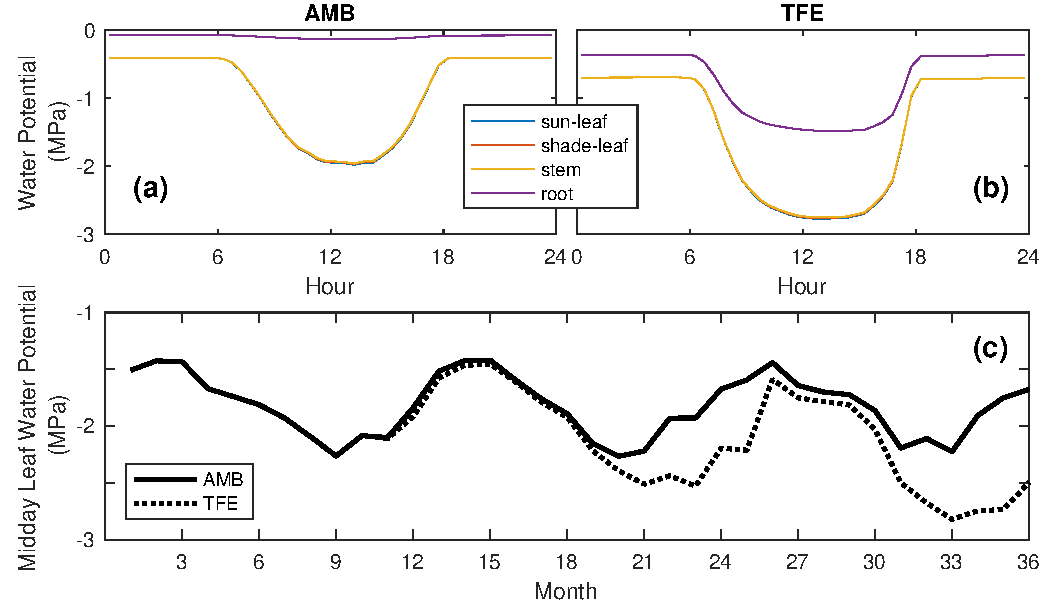
\includegraphics[width=30pc]{../figs2/fig2.pdf}
     \caption{Modeled vegetation water potential at  Caxiuan\~a, Brazil.
     (a) 2003 Dry season (SON) diurnal mean, ambient throughfall conditions,
     (b) 2003 Dry season (SON) diurnal mean, with 60\% throughfall excluded.
     Curves are drawn for sunlit leaf, shaded leaf, stem, and root water potentials. Note that the first three mostly overlap.
     (c) Monthly mean midday leaf water potential, under ambient (solid line) and 60\% throughfall exclusion (dotted line) conditions.
     Note that throughfall exclusion begins in month 11 (Nov 1, 2001).
     }
     \label{fig:vwp}
  \end{figure}
  
  \clearpage   
  \begin{figure}[h]
     \centering
     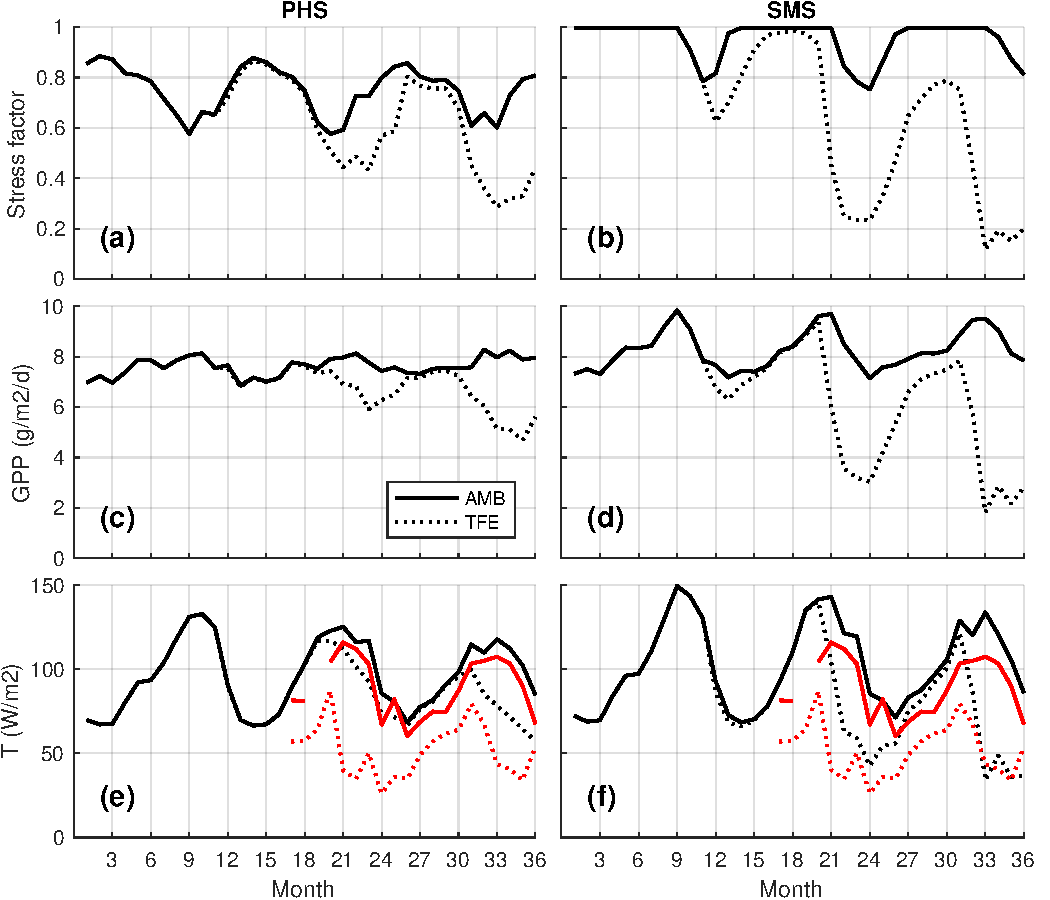
\includegraphics[width=30pc]{../figs2/fig3.pdf}
     \caption{(a,b) Monthly mean water stress function. Note that the water stress function equals 1 when there is no stress and 0 when fully stressed.
     (c,d) Monthly mean transpiration (W/m$^2$).
     (e,f) Monthly mean gross primary productivity (g/m$^2$/d). 
     Solid lines correspond to ambient throughfall conditions, and dotted lines feature 60\% throughfall exclusion.
     Black lines represent model output.
     Red lines show observational transpiration derived from sap flux (see zqz).
     PHS is on for (a), (c), and (e). PHS is off for (b), (d), and (f).
     }
     \label{fig:mm}
  \end{figure}
  
          \clearpage
    \begin{figure}[h]
     \centering
     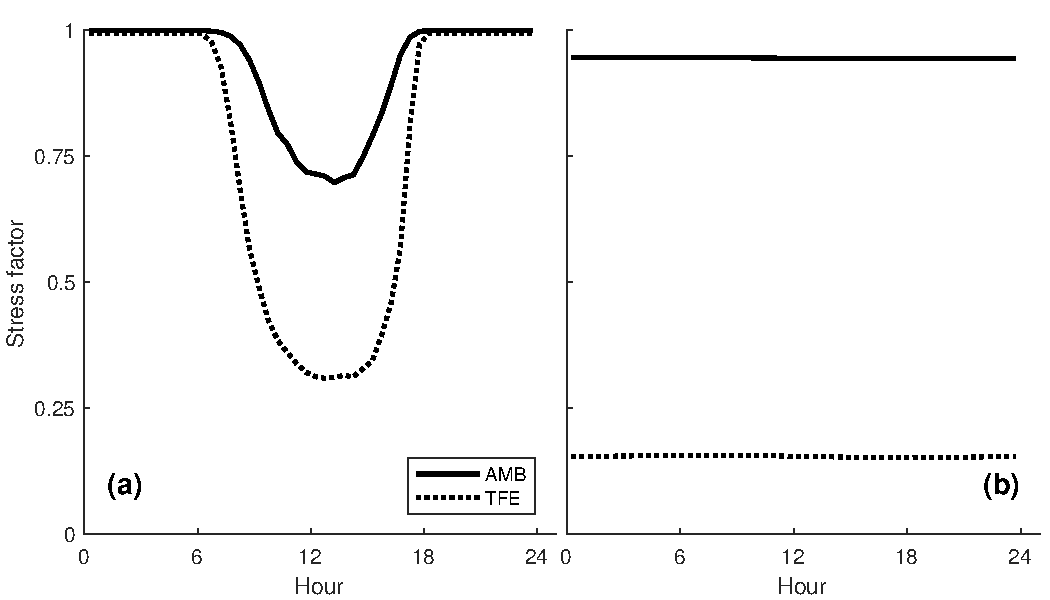
\includegraphics[width=30pc]{../figs2/fig4.pdf}
     \caption{2003 Dry season (SON) diurnal mean water stress function for 
     (a) PHS on, and
     (b) PHS off.
     Solid lines correspond to ambient throughfall conditions, and dotted lines feature 60\% throughfall exclusion.
     Note that the water stress function equals 1 when there is no stress and 0 when fully stressed.
     }
     \label{fig4}
  \end{figure}
  
      \clearpage
    \begin{figure}[h]
     \centering
     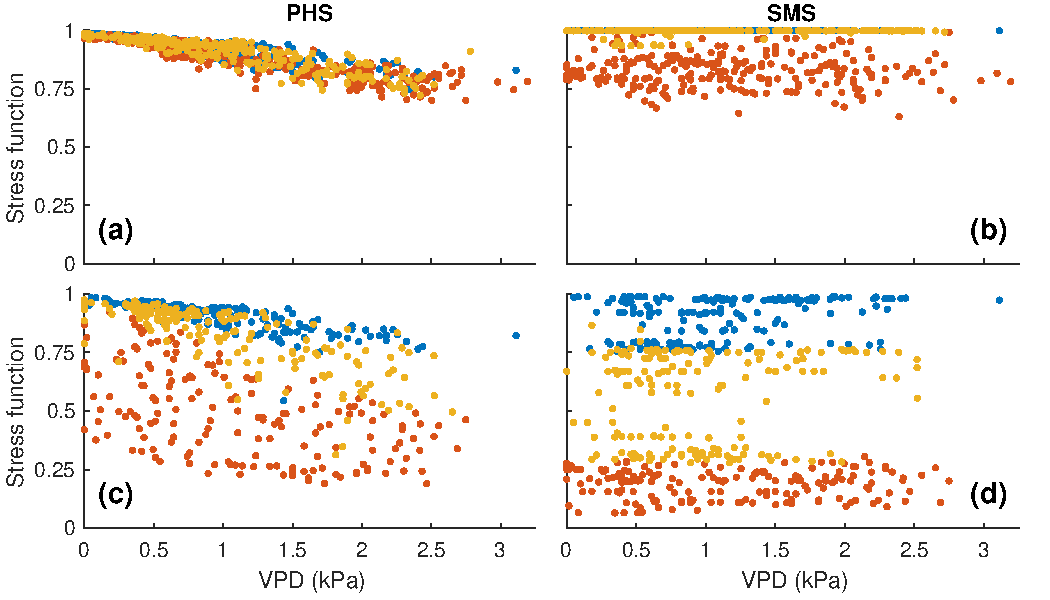
\includegraphics[width=30pc]{../figs2/fig5.pdf}
     \caption{Water stress function versus vapor pressure deficit, for points with downwelling shortwave radiation between 400 and 425 W/m2.
     (a) PHS, ambient throughfall
     (b) SMS, ambient throughfall
     (c) PHS, 60\% throughfall excluded
     (d) SMS, 60\% throughfall excluded. 
     For (a) and (c) data are subdivided based on predawn root water potential.
     For (b) and (d) data are subdivided based on average soil matric potential, weighted by root fraction.
     Blue dots represent the wettest tercile, yellow dots represent the intermediate tercile, and red dots represent the driest tercile.
     Note that panels (c) and (d) exclude data from 2001, when throughfall exclusion was not active.
     }
     \label{fig:vpd}
       \end{figure}
  
  
\clearpage   
  \begin{figure}[h]
     \centering
     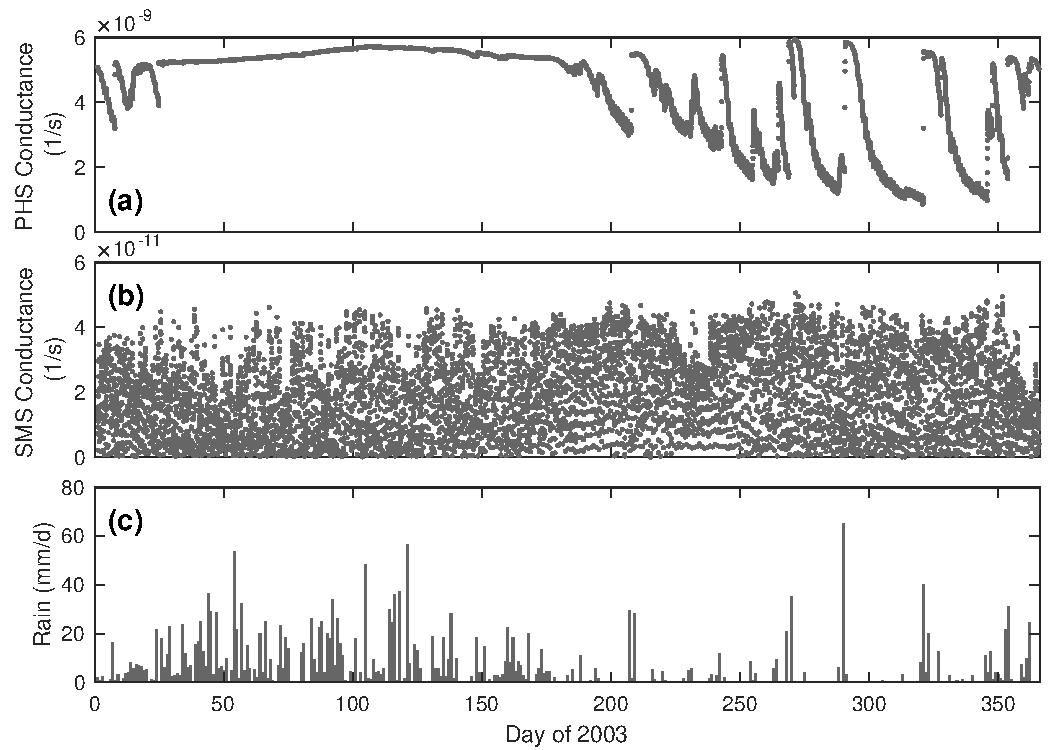
\includegraphics[width=30pc]{../figs2/fig6.pdf}
     \caption{Soil Layer 3 conductance, under ambient throughfall conditions in 2003. 
     (a) Time-series of PHS modeled soil-to-root conductance (s$^{-1}$) from Soil Layer 3 (spanning 6 to 12 centimeters in depth).
     (b) Time-series of SMS inferred conductance (s$^{-1}$) also from Soil Layer 3.
     (c) Concurrent precipitation forcing (mm/d).
     }
     \label{fig:cond}
  \end{figure}
  
  \clearpage   
  \begin{figure}[h]
     \centering
     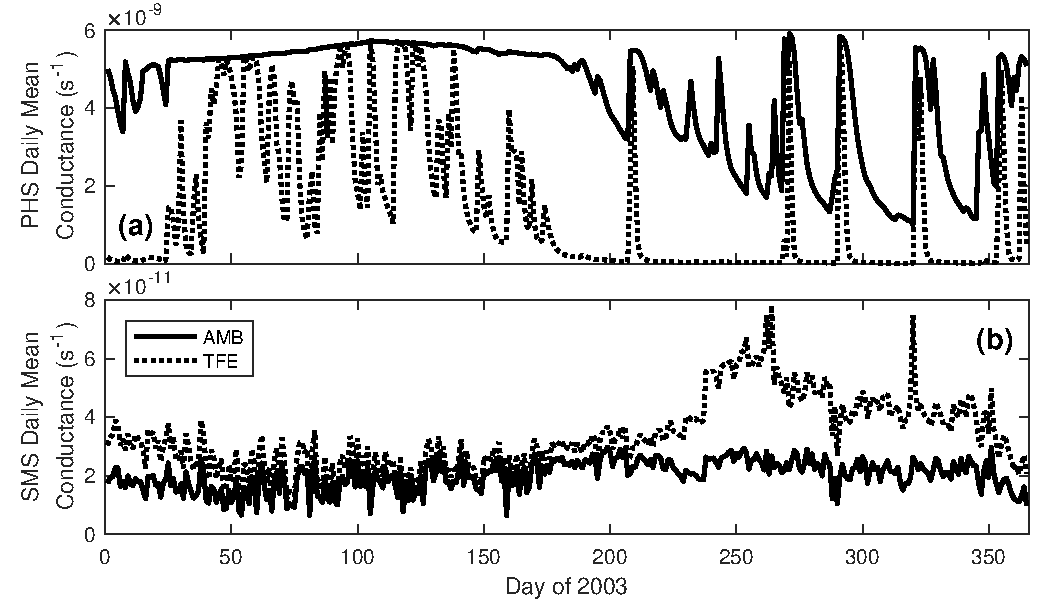
\includegraphics[width=30pc]{../figs2/fig6a.pdf}
     \caption{Daily mean Soil Layer 3 conductance, throughout 2003 under ambient (solid line) and 60\% throughfall exclusion (dotted line) conditions.
     (a) Daily mean of PHS modeled soil-to-root conductance (s$^{-1}$) from Soil Layer 3 (spanning 6 to 12 centimeters in depth).
     (b) Daily mean of SMS inferred conductance (s$^{-1}$) also from Soil Layer 3.
     }
     \label{fig:cond2}
  \end{figure}
  
        \clearpage
    \begin{figure}[h]
     \centering
     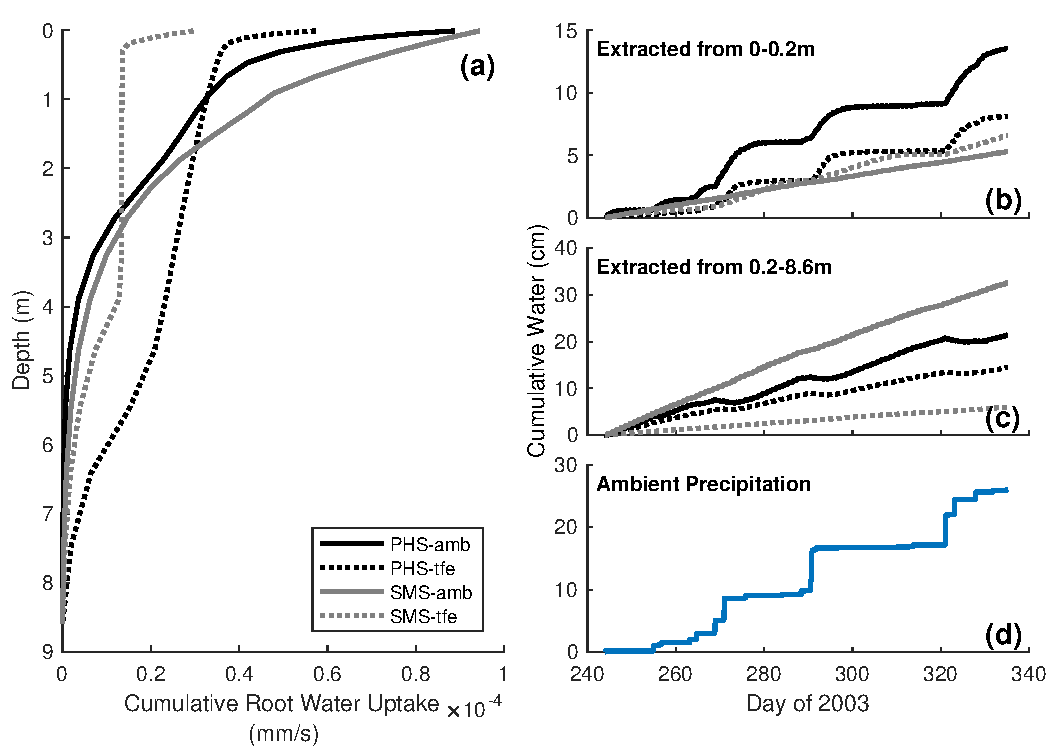
\includegraphics[width=30pc]{../figs2/fig7.pdf}
     \caption{2003 dry season (SON) root water uptake. 
     Panel (a) shows the average cumulative profile of root water uptake rate (mm/s) for the four simulations over SON-2003.
     Panel (b) shows cumulative total  water uptake from above 0.2m for the four simulations during SON-2003.
     Panel (c) shows cumulative total water uptake from below 0.2m for the four simulations during SON-2003. 
     Panel (d) shows cumulative total ambient precipitation during SON-2003.
     }
     \label{fig7}
  \end{figure}
  
        \clearpage
    \begin{figure}[h]
     \centering
     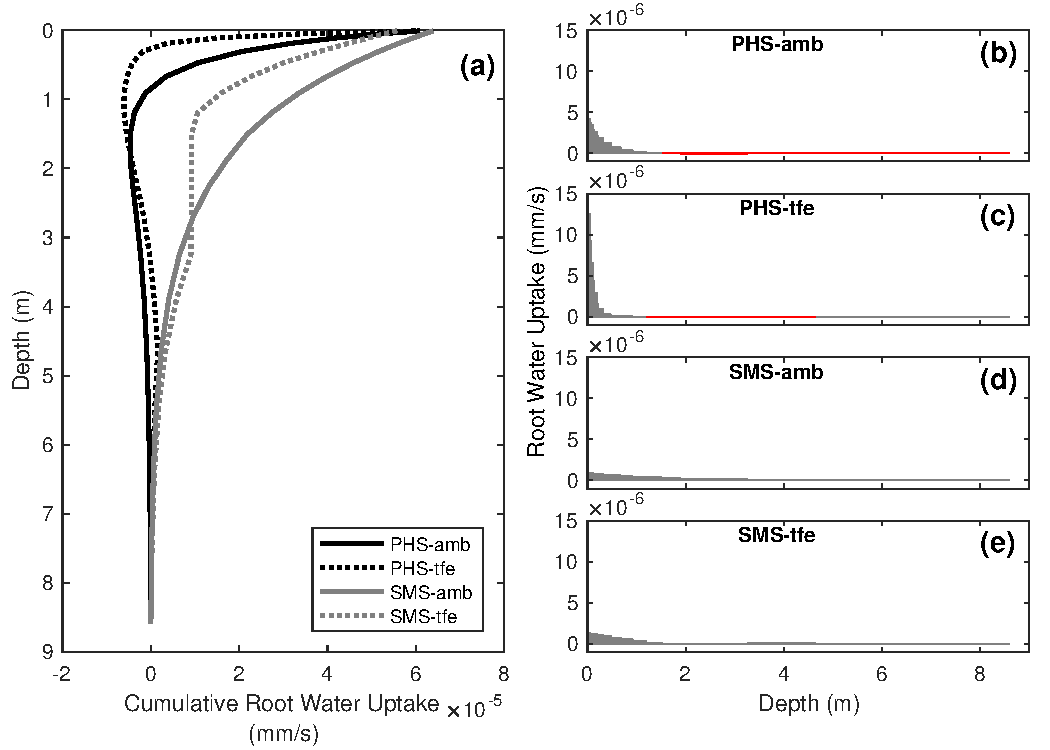
\includegraphics[width=30pc]{../figs2/fig8.pdf}
     \caption{2003 wet season (FMA) root water uptake. 
     Panel (a) shows the average cumulative profile of root water uptake rate (mm/s) for the four simulations over FMA-2003.
     Panel (b) shows cumulative total water uptake from above 0.2m for the four simulations during FMA-2003.
     Panel (c) shows cumulative total water uptake from below 0.2m for the four simulations during FMA-2003. 
     Panel (d) shows cumulative total ambient precipitation during FMA-2003. 
     }
     \label{fig8}
  \end{figure}
  
    \clearpage
    \begin{figure}[h]
     \centering
     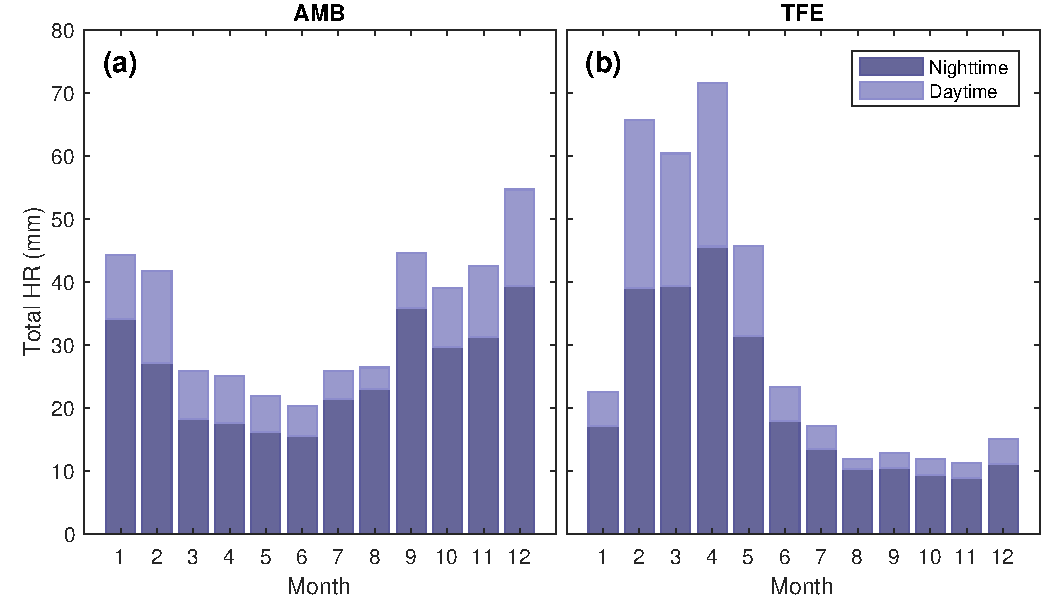
\includegraphics[width=30pc]{../figs2/fig9.pdf}
     \caption{Total hydraulic redistribution (mm) by month in 2003. For (a) ambient throughfall conditions, and (b) 60\% throughfall exclusion. 
     Darker shading shows portion of HR at night [6pm,6am), lighter shading shows portion of HR during day [6am,6pm).}
     \label{fig:hr}
  \end{figure}

  
      \clearpage
    \begin{figure}[h]
     \centering
     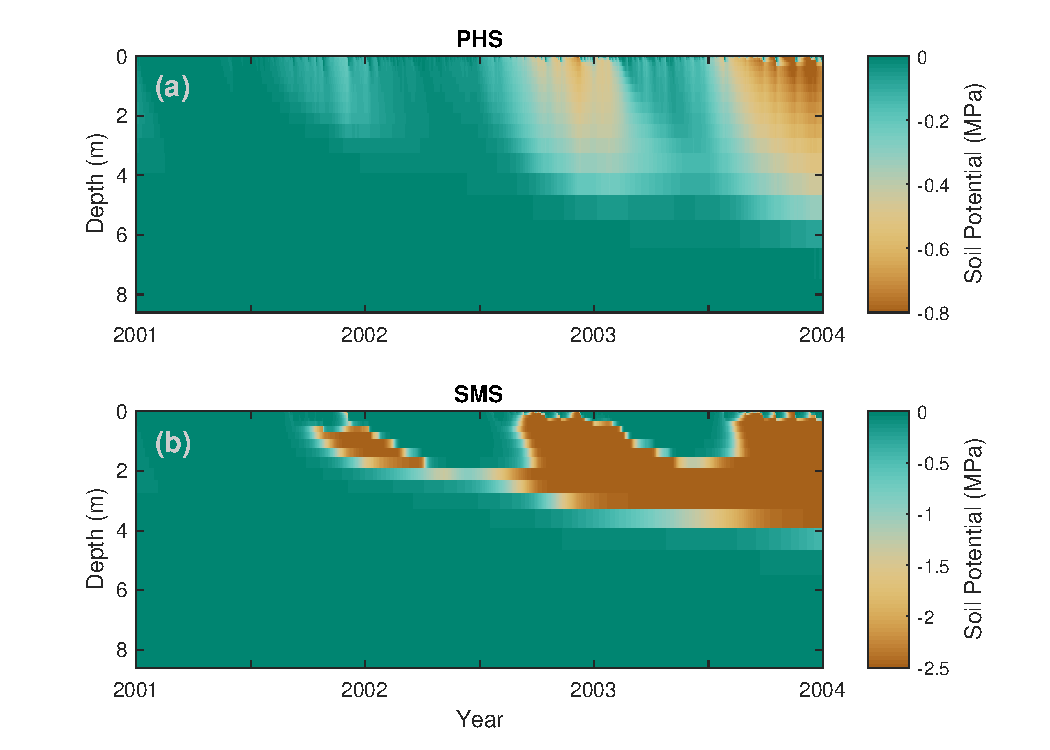
\includegraphics[width=30pc]{../figs2/fig11.pdf}
     \caption{Vertical profile of soil water potential (MPa) over time under 60\% throughfall exclusion, for
     (a) PHS, and 
     (b) SMS.
     Note that color axes are different. }
     \label{fig11}
  \end{figure}


\clearpage

\appendix
%====================
%  APPENDIX
%====================

\section{Supplementary Figures}

      \begin{figure}[h]
     \centering
     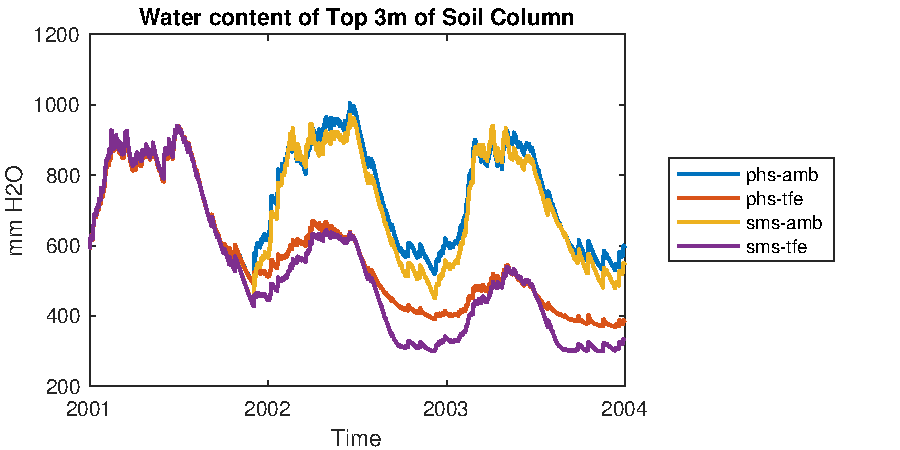
\includegraphics[width=30pc]{../figs2/top3m.pdf}
     \caption{Total water content of the top three meters of the soil column through time for the four simulations.}
     \label{top3m}
  \end{figure}
  \clearpage
  
      \begin{figure}[h]
     \centering
     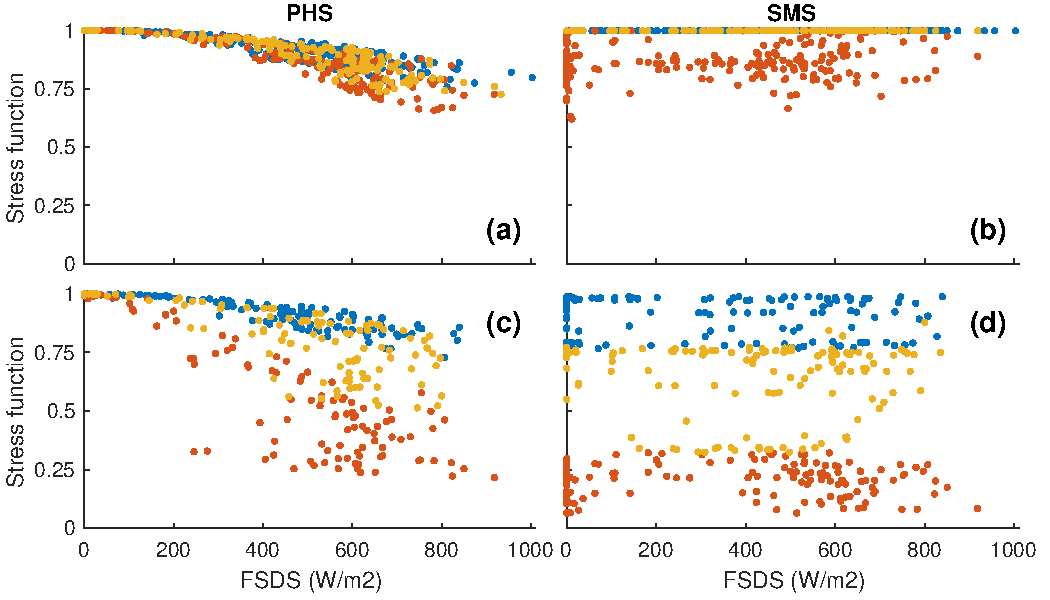
\includegraphics[width=30pc]{../figs2/suppfsds.pdf}
     \caption{Water stress function versus downwelling shortwave radiation for points with vapor pressure deficit between 1 and 1.0559 kPa.
     (a) PHS, ambient throughfall
     (b) SMS, ambient throughfall
     (c) PHS, 60\% throughfall excluded
     (d) SMS, 60\% throughfall excluded. 
     For (a) and (c) data are subdivided based on predawn root water potential.
     For (b) and (d) data are subdivided based on average soil matric potential, weighted by root fraction.
     Blue dots represent the wettest tercile, yellow dots represent the intermediate tercile, and red dots represent the driest tercile.
     Note that panels (c) and (d) exclude data from 2001, when throughfall exclusion was not active.
     }
     \label{supp:fsds}
       \end{figure}
  
        \begin{figure}[h]
     \centering
     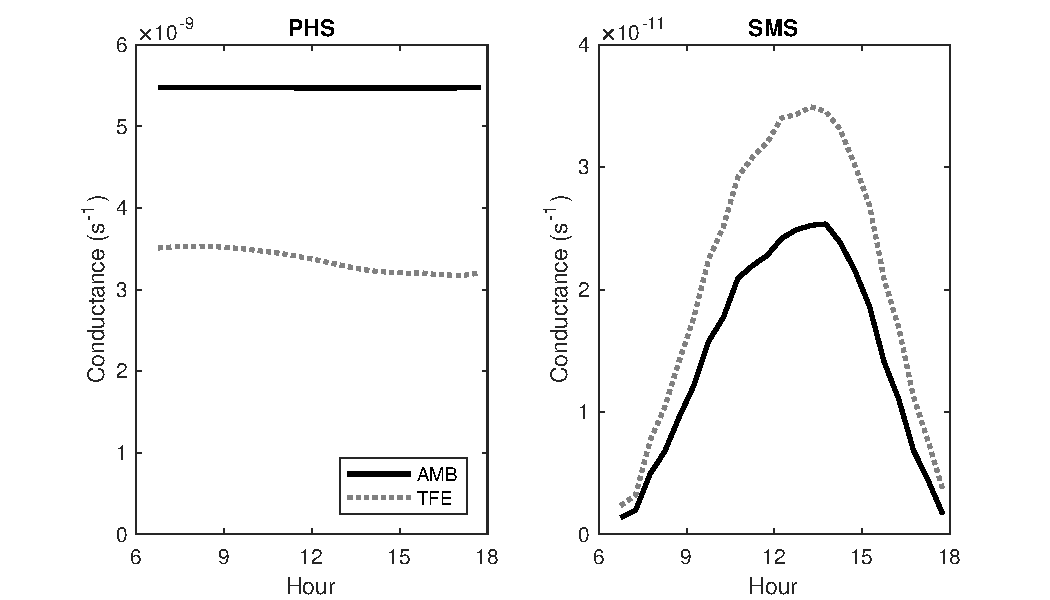
\includegraphics[width=30pc]{../figs2/suppfig1.pdf}
     \caption{FMA-2003 average diurnal cycle of layer 3 conductance.}
     \label{supp:cond}
  \end{figure}
  \clearpage
  
  \begin{figure}[h]
     \centering
     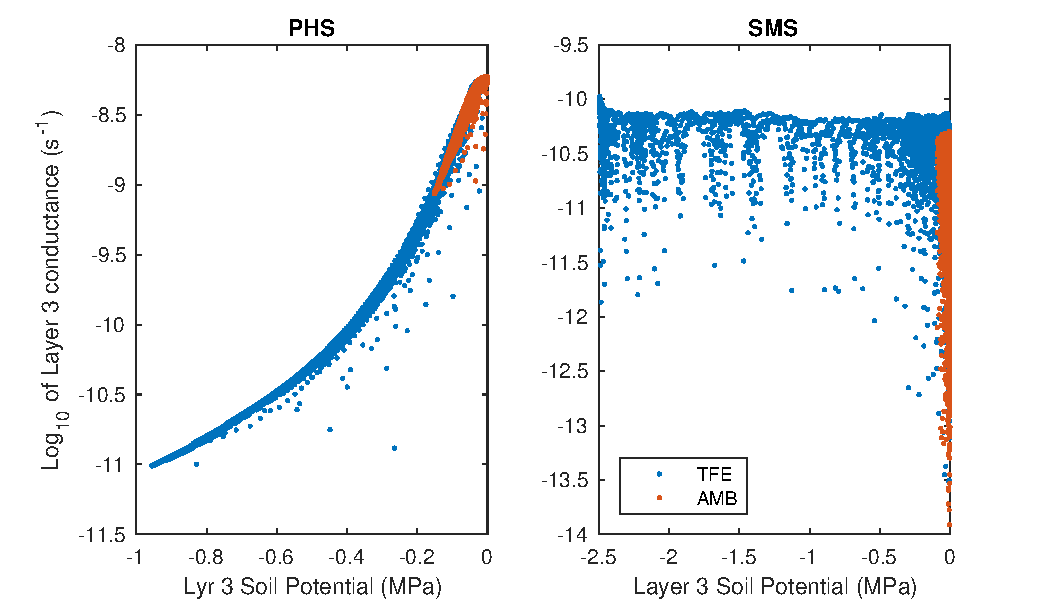
\includegraphics[width=30pc]{../figs2/suppfig2.pdf}
     \caption{Log of conductance versus soil potential for Soil Layer 3 (2003).}
     \label{supp:cond2}
  \end{figure}
  \clearpage

    \begin{figure}[h]
     \centering
     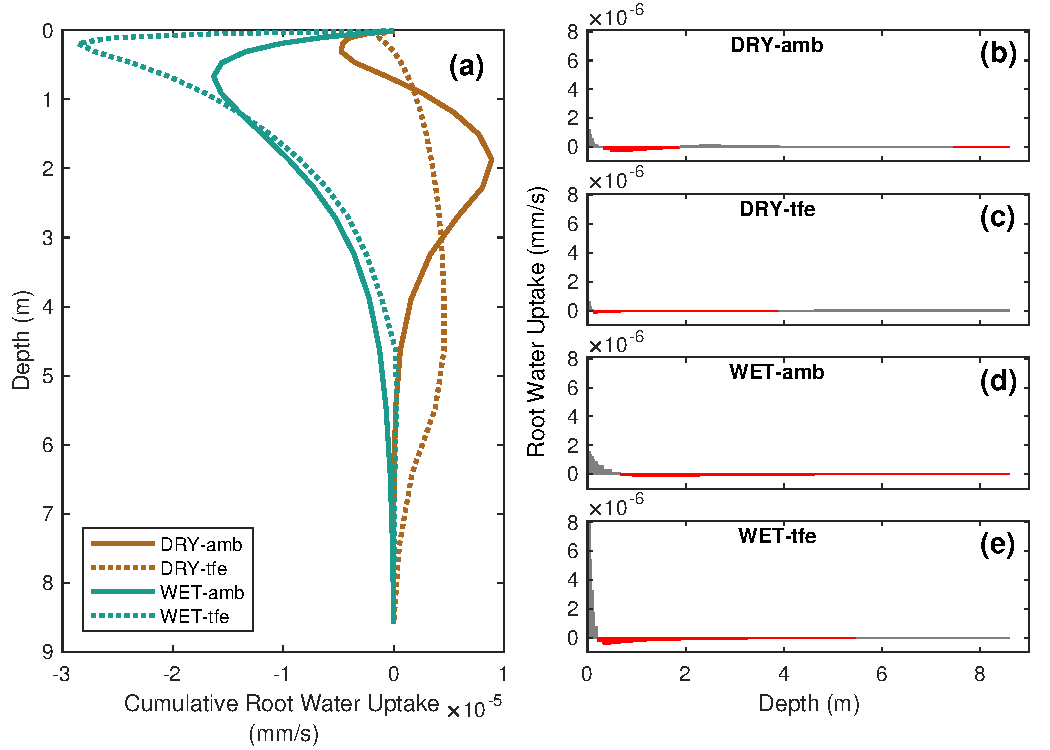
\includegraphics[width=30pc]{../figs2/fig10.pdf}
     \caption{PHS, nighttime (6pm to 6am) average root water uptake profiles with depth. 
     Showing nighttime serves to emphasize the profile of hydraulic redistribution.
     Panel (a) shows cumulative (starting at depth) root water uptake (mm/s) for ambient (solid line) and 60\% throughfall exclusion (dotted line)
     during the wet (FMA, cyan color) and dry (SON, brown color) seasons. 
     Panels (b)-(e) present the information from (a) in non-cumulative form. 
     Note that for panels (b)-(e) negative root water uptake is shaded red, and also that for panel (a), 
     positive slope indicates water uptake, and negative slope indicates water deposited.
     Note also that SMS is not shown, because hydraulic redistribution is precluded.}
     \label{supp:hr}
  \end{figure}
  \clearpage
  
      \begin{figure}[h]
     \centering
     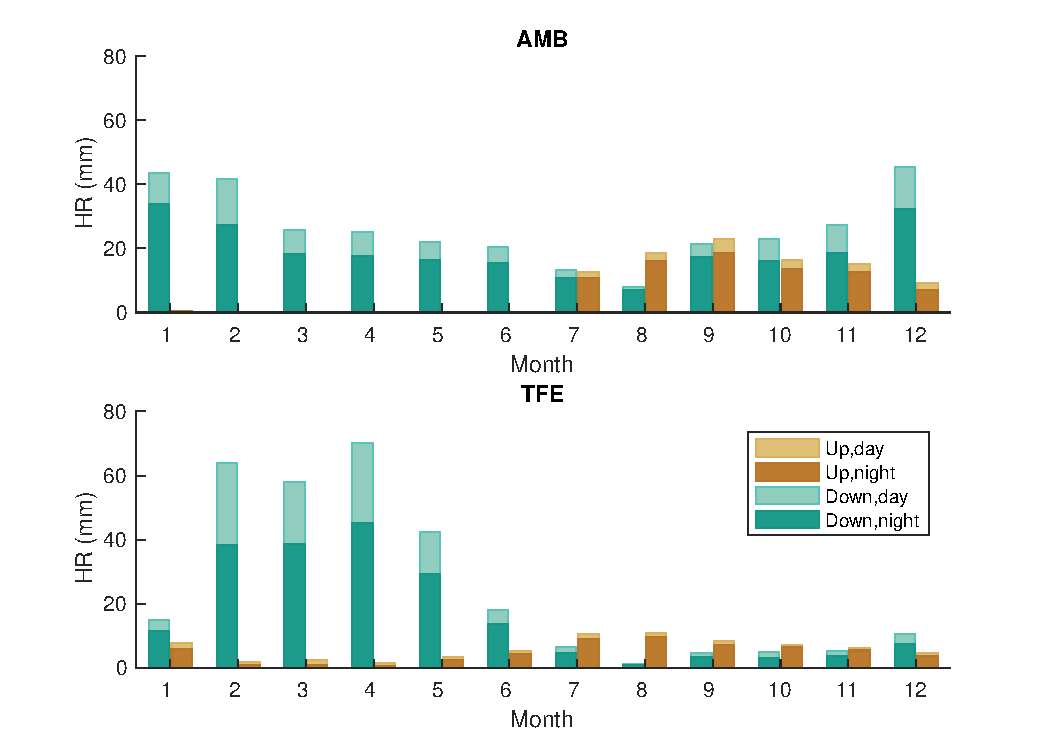
\includegraphics[width=30pc]{../figs2/supphr.pdf}
     \caption{PHS hydraulic distribution during 2003. Alternative version partitioning by direction.}
     \label{supp:hr2}
  \end{figure}
  \clearpage
  
     \clearpage
    \begin{figure}[h]
     \centering
     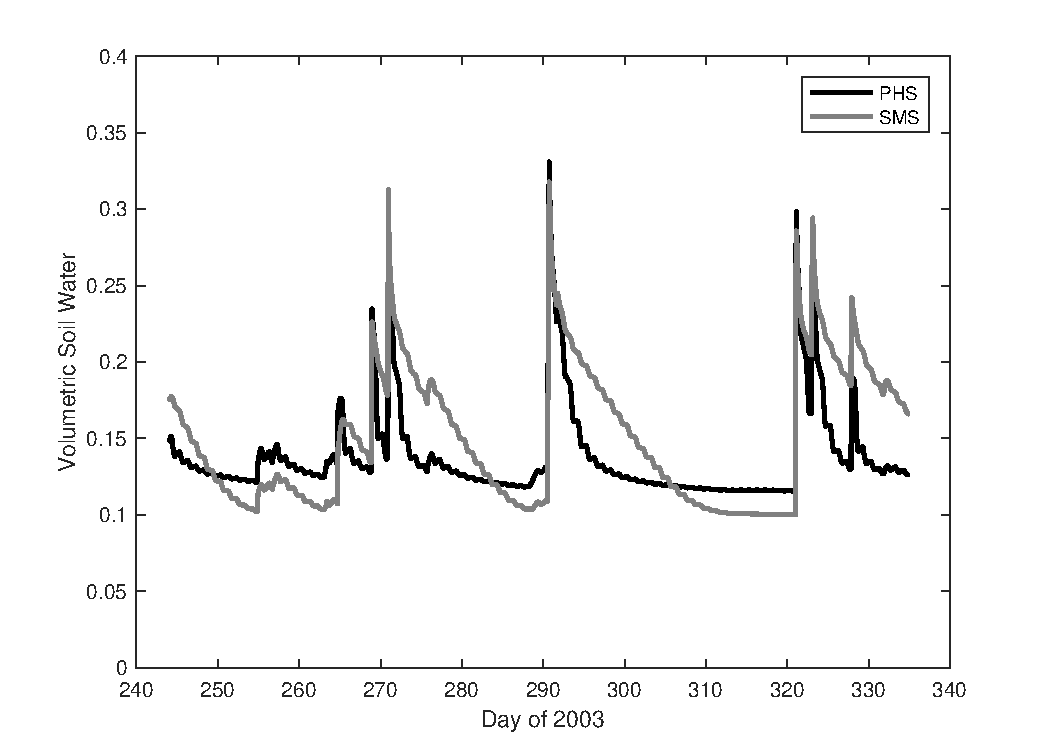
\includegraphics[width=30pc]{../figs2/supplayer2.pdf}
     \caption{Volumetric soil water content in Soil Layer 2 (which spans 2-6cm in depth), for SON-2003, featuring 60\% throughfall exclusion.
     With PHS (black line), the soil layer can dry out much more quickly after rain events.}
     \label{supp:layer2}
  \end{figure}

        \clearpage
    \begin{figure}[h]
     \centering
     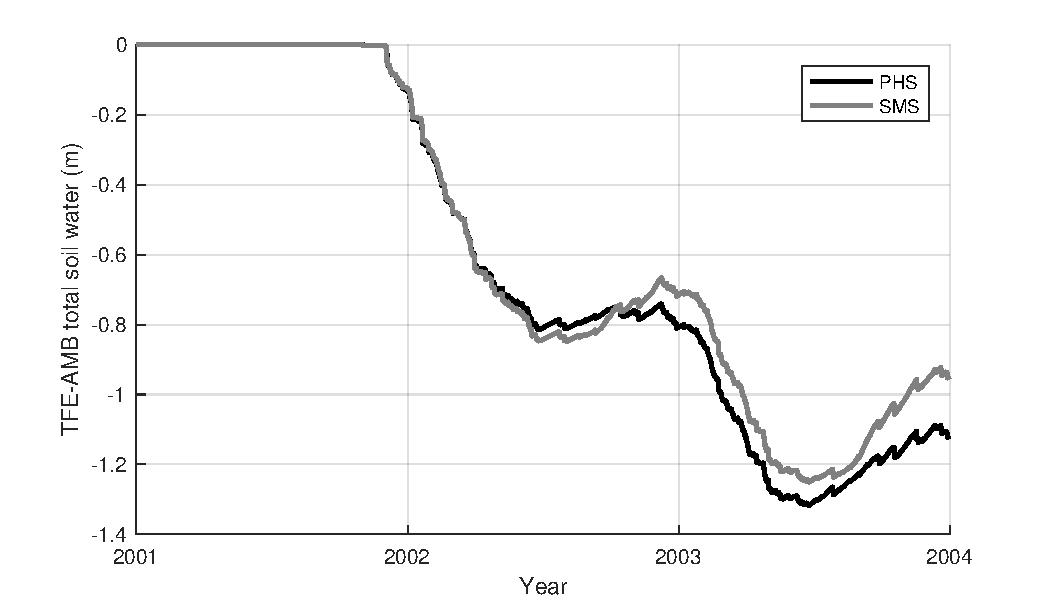
\includegraphics[width=30pc]{../figs2/suppsoilwater.pdf}
     \caption{Delta soil water}
     \label{supp:buff}
  \end{figure}
  
  
        \clearpage
    \begin{figure}[h]
     \centering
     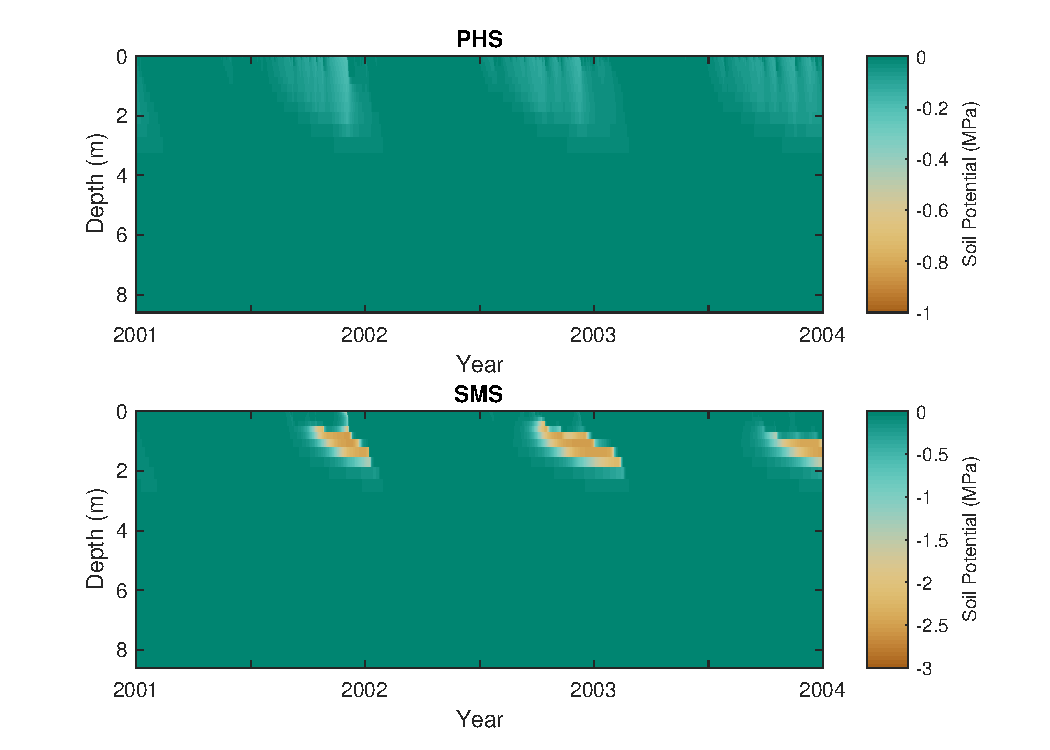
\includegraphics[width=30pc]{../figs2/suppsmp.pdf}
     \caption{Vertical profile of soil water potential (MPa) through time under ambient throughfall conditions, for
     (a) PHS, and 
     (b) SMS.
     Note that color axes are different. }
     \label{supp:smp}
  \end{figure}



\section{Appendix to Model Description}

% Details on water supply
\subsection{Details of Water Supply}

PHS resolves flow across four different segments, soil-to-root, root-to-stem, stem-to-leaf, and leaf-to-transpiration.

Stem-to-leaf. The area bases are sunlit and shaded leaf area, respectively. 
Note that gravity is assumed negligible here. 
Likewise there is no length scaling applied to maximum conductance. 
Therefore the input parameters for $k_{1,\text{max}}$ should be conductances ($s^{-1}$).

\begin{linenomath*} \begin{equation} \begin{aligned}
q_{1a} &= k_{1} \cdot \text{LAI-sun}  \cdot \left( \psi_{\text{stem}}-\psi_{\text{sun-leaf}}\right) \\
q_{1b} &= k_{1} \cdot \text{LAI-shade} \cdot  \left( \psi_{\text{stem}}-\psi_{\text{shade-leaf}}\right)
\end{aligned} \end{equation} \end{linenomath*}

\begin{linenomath*} \begin{equation}
k_{1} = k_{1,\text{max}} \cdot f\left(\psi_{\text{stem}}\right)
\end{equation} \end{linenomath*}

\begin{linenomath*} \begin{equation} \begin{aligned}
f\left(\psi\right)=2^{-\left(\dfrac{\psi}{p_{50}}\right)^{c_k}}
\end{aligned} \end{equation} \end{linenomath*}

Root-to-stem. The area basis is stem area index. 
The parameter is maximum stem xylem conductivity ($K_{2,\text{max}}$).
Stem conductance ($k_2$) is the result of scaling maximum conductivity by the tree height ($h$)
and applying loss relative to maximum conductance via the vulnerability curve $f\left(\psi_{\text{root}}\right)$. 
\begin{linenomath*} \begin{equation}
q_2 = k_2 \cdot  \text{SAI}  \cdot \left( \psi_{\text{root}}-\psi_{\text{stem}}-\rho g h\right)
\end{equation} \end{linenomath*}
\begin{linenomath*} \begin{equation}
k_2 = \dfrac{K_{2,\text{max}}}{h} \cdot f\left(\psi_{\text{root}}\right)
\end{equation} \end{linenomath*}

Soil-to-root. Area basis is RAI in soil layer $i$, which is based on the layer root fraction times the
total root area. Total root area we have as the summed stem and leaf area indices multiplied by a relative
root area parameter ($f_{\text{root}}$).
The vertical root distribution is defined by the layer root fraction ($r_i$), which follows a one-parameter 
(by PFT) power law decay following \citet{jackson1996}.

\begin{linenomath*} \begin{equation}
q_{3,i} = k_{3,i} \cdot  \text{RAI}_i  \cdot \left( \psi_{\text{soil,i}}-\psi_{\text{root}}-\rho g z_i\right)
\end{equation} \end{linenomath*}
\begin{linenomath*} \begin{equation}
\text{RAI}_i=f_{\text{root}} \cdot \left( \text{SAI} + \text{LAI} \right) \cdot r_i
\label{eq:rai}
\end{equation} \end{linenomath*}
\begin{linenomath*} \begin{equation}
k_{3,i} = \dfrac{k_{r,i}+k_{s,i}}{k_{r,i}\cdot k_{s,i}}
\end{equation} \end{linenomath*}
\begin{linenomath*} \begin{equation}
k_{r,i} = \dfrac{K_{r,\text{max}}}{l_i} f \left(\psi_{\text{soil,i}}\right)
\end{equation} \end{linenomath*}
\begin{linenomath*} \begin{equation}
l_i = z_i + x
\end{equation} \end{linenomath*}
\begin{linenomath*} \begin{equation}
k_{s,i} = \dfrac{K_{s,i}}{d}
\end{equation} \end{linenomath*}

The conductance $k_{3,i}$ reflects two resistors in series, from soil-to-root ($k_{s,i}$) and through the
root tissue ($k_{r,i}$).
The root tissue conductance is attenuated via the vulnerability curve framework. 
The input parameter is maximum root xylem conductivity, on the basis of RAI as defined above.
The root conductivity is scaled by the conducting length, which is estimated as the sum of soil layer depth ($z_i$)
and average lateral extent ($x$, static parameter).
The soil conductivity $K_{s,i}$ is calculated from the layer soil matric potential ($\psi_s$) 
and soil properties following \citet{clapp1978} as described in \citet{oleson2013}.
The soil conductance ($k_{s,i}$) is the result of scaling the conductivity by $d$, 
 the distance between roots estimated following \citet{williams1996} and \citet{bonan2014}

The challenge here is obviously getting your head around all the parameters.

% Details on water demand
\subsection{Details of Water Demand}

% Details on phs solution
\subsection{Details of Solution}


The continuity of water flow through the system yields four equations
   \begin{linenomath*} \begin{equation}
   \begin{aligned}
   E_{sun}&=q_{1a}\\
   E_{shade}&=q_{1b}\\
   q_{1a}+q_{1b}&=q_2\\
   q_2&=\sum_{i=1}^{nlevsoi}{q_{3,i}}
   \end{aligned}
   \end{equation} \end{linenomath*}

We seek the set of vegetation water potential values (four unknowns), 

   \begin{linenomath*} \begin{equation}
   \psi=\left[ \begin {array}{c} 
   \psi_{sunleaf}\cr\psi_{shadeleaf}\cr\psi_{stem}\cr\psi_{root}
   \end {array} \right] 
   \end{equation} \end{linenomath*}

that satisfies these equations, as forced by the soil moisture and atmospheric state. 

Each flux on the schematic can be represented in terms of the relevant water potentials. 

Defining the transpiration fluxes:


   \begin{linenomath*} \begin{equation}
   \begin{aligned}
   E_{sun} &= E_{sun,max} \cdot 2^{-\left(\dfrac{\psi_{sunleaf}}{p50_e}\right)^{c_k}} \\
   E_{shade} &= E_{shade,max} \cdot 2^{-\left(\dfrac{\psi_{shadeleaf}}{p50_e}\right)^{c_k}} 
   \end{aligned}
   \end{equation} \end{linenomath*}

Defining the water supply fluxes:

   \begin{linenomath*} \begin{equation}
   \begin{aligned}
   q_{1a}&=k_{1a,max}\cdot 2^{-\left(\dfrac{\psi_{stem}}{p50_1}\right)^{c_k}} \cdot\mbox{LAI}_{sun}\cdot\left(\psi_{stem}-\psi_{sunleaf} \right) \\
   q_{1b}&=k_{1b,max}\cdot 2^{-\left(\dfrac{\psi_{stem}}{p50_1}\right)^{c_k}}\cdot\mbox{LAI}_{shade}\cdot\left(\psi_{stem}-\psi_{shadeleaf} \right) \\
   q_2&=\dfrac{k_{2,max}}{z_2} \cdot 2^{-\left(\dfrac{\psi_{root}}{p50_2}\right)^{c_k}} \cdot SAI \cdot \left( \psi_{root} - \psi_{stem} - \Delta \psi_z  \right) \\
   q_{soil}&=\sum_{i=1}^{nlevsoi}{q_{3,i}}=\sum_{i=1}^{nlevsoi}{k_{3,i}\cdot RAI\cdot\left(\psi_{soil,i}-\psi_{root} + \Delta\psi_{z,i} \right)}
   \end{aligned}
   \end{equation} \end{linenomath*}

We're looking to find the vector $\psi$
that fits with soil and atmospheric forcings while satisfying water flow continuity. 
Due to the model non-linearity, we use a linearized explicit approach, iterating with Newton's method. 
The initial guess is the solution for $\psi$ (vector) from the previous time step. 
The general framework, from iteration $m$ to $m+1$ is:

   \begin{linenomath*} \begin{equation} 
   \begin{aligned}
   q^{m+1}&=q^m+\dfrac{\delta q}{\delta\psi}\Delta\psi \\
   \psi^{m+1}&=\psi^{m}+\Delta\psi
   \end{aligned}
   \end{equation} \end{linenomath*}

So for our first flux balance equation, at iteration $m+1$, we have:

   \begin{linenomath*} \begin{equation} 
   E_{sun}^{m+1}=q_{1a}^{m+1}
   \end{equation} \end{linenomath*}

Which can be linearized to:

   \begin{linenomath*} \begin{equation} 
   E_{sun}^{m}+\dfrac{\delta E_{sun}}{\delta\psi}\Delta\psi=q_{1a}^{m}+\dfrac{\delta q_{1a}}{\delta\psi}\Delta\psi
   \end{equation} \end{linenomath*}

And rearranged to be:

   \begin{linenomath*} \begin{equation} 
   \dfrac{\delta q_{1a}}{\delta\psi}\Delta\psi-\dfrac{\delta E_{sun}}{\delta\psi}\Delta\psi=E_{sun}^{m}-q_{1a}^{m}
   \end{equation} \end{linenomath*}

And for the other 3 flux balance equations:

   \begin{linenomath*} \begin{equation} 
   \begin{aligned}
   \dfrac{\delta q_{1b}}{\delta\psi}\Delta\psi-\dfrac{\delta E_{sha}}{\delta\psi}\Delta\psi&=E_{sha}^{m}-q_{1b}^{m} \\
   \dfrac{\delta q_2}{\delta\psi}\Delta\psi-\dfrac{\delta q_{1a}}{\delta\psi}\Delta\psi-\dfrac{\delta q_{1b}}{\delta\psi}\Delta\psi&=q_{1a}^{m}+q_{1b}^{m}-q_2^{m} \\
   \dfrac{\delta q_{soil}}{\delta\psi}\Delta\psi-\dfrac{\delta q_2}{\delta\psi}\Delta\psi&=q_2^{m}-q_{soil}^{m}
   \end{aligned}
   \end{equation} \end{linenomath*}

Putting all four together in matrix form:

   \begin{linenomath*} \begin{equation} 
   \left[ \begin {array}{c}
   \dfrac{\delta q_{1a}}{\delta\psi}-\dfrac{\delta E_{sun}}{\delta\psi} \cr
   \dfrac{\delta q_{1b}}{\delta\psi}-\dfrac{\delta E_{sha}}{\delta\psi} \cr
   \dfrac{\delta q_2}{\delta\psi}-\dfrac{\delta q_{1a}}{\delta\psi}-\dfrac{\delta q_{1b}}{\delta\psi} \cr
   \dfrac{\delta q_{soil}}{\delta\psi}-\dfrac{\delta q_2}{\delta\psi}
   \end {array} \right]
   \Delta\psi=
   \left[ \begin {array}{c}
   E_{sun}^{m}-q_{1a}^{m} \cr
   E_{sha}^{m}-q_{1b}^{m} \cr
   q_{1a}^{m}+q_{1b}^{m}-q_2^{m} \cr
   q_2^{m}-q_{soil}^{m}
   \end {array} \right]
   \end{equation} \end{linenomath*}

Now to expand the left-hand side, from vector $\psi$ to the four distinct plant water potential nodes, noting that many derivatives are zero (e.g. $\dfrac{\delta E_{sun}}{\delta\psi_{sha}}=0$)

Introducing the notation:
$A\Delta\psi=b$

   \begin{linenomath*} \begin{equation} 
   \Delta\psi=\left[ \begin {array}{c}
   \Delta\psi_{sunleaf} \cr
   \Delta\psi_{shadeleaf} \cr
   \Delta\psi_{stem} \cr
   \Delta\psi_{root}
   \end {array} \right] 
   \end{equation} \end{linenomath*}

   \begin{linenomath*} \begin{equation} 
   A=
   \left[ \begin {array}{cccc}
   \dfrac{\delta q_{1a}}{\delta \psi_{sun}}-\dfrac{\delta E_{sun}}{\delta \psi_{sun}}&0&\dfrac{\delta q_{1a}}{\delta \psi_{stem}}&0\cr
   0&\dfrac{\delta q_{1b}}{\delta \psi_{sha}}-\dfrac{\delta E_{sha}}{\delta \psi_{sha}}&\dfrac{\delta q_{1b}}{\delta \psi_{stem}}&0\cr
   -\dfrac{\delta q_{1a}}{\delta \psi_{sun}}&
   -\dfrac{\delta q_{1b}}{\delta \psi_{sha}}&
   \dfrac{\delta q_2}{\delta \psi_{stem}}-\dfrac{\delta q_{1a}}{\delta \psi_{stem}}-\dfrac{\delta q_{1b}}{\delta \psi_{stem}}&
   \dfrac{\delta q_2}{\delta \psi_{root}}\cr
   0&0&-\dfrac{\delta q_2}{\delta \psi_{stem}}&\dfrac{\delta q_{soil}}{\delta \psi_{root}}-\dfrac{\delta q_2}{\delta \psi_{root}}
   \end {array} \right]
   \end{equation} \end{linenomath*}

   \begin{linenomath*} \begin{equation} 
   b=
   \left[ \begin {array}{c}
   E_{sun}^{m}-q_{b1}^{m} \cr
   E_{sha}^{m}-q_{b2}^{m} \cr
   q_{b1}^{m}+q_{b2}^{m}-q_{stem}^{m} \cr
   q_{stem}^{m}-q_{soil}^{m}
   \end {array} \right]
   \end{equation} \end{linenomath*}

Now we compute all the entries for $A$ and $b$ based on the soil moisture and maximum transpiration forcings and can solve to find:

   \begin{linenomath*} \begin{equation} 
   \Delta\psi=A^{-1}b
   \end{equation} \end{linenomath*}

   \begin{linenomath*} \begin{equation} 
   \psi_{m+1}=\psi_m+\Delta\psi
   \end{equation} \end{linenomath*}

We iterate until $b\to 0$, signifying water flux balance through the system. The result is a final set of water potentials ( $\psi_{root}$, $\psi_{xylem}$, $\psi_{shadeleaf}$, $\psi_{sunleaf}$) satisfying non-divergent water flux through the system. 
The magnitude of the water flux is driven by soil matric potential and unstressed ( $\beta_t=1$) transpiration. 

We use the transpiration solution (corresponding to the final solution for $\psi$) to compute stomatal conductance. The stomatal conductance is then used to compute $\beta_t$. 

   \begin{linenomath*} \begin{equation} 
   \beta_{t,sun} = \dfrac{g_{s,sun}}{g_{s,sun,\beta_t=1}} 
   \end{equation} \end{linenomath*}

   \begin{linenomath*} \begin{equation} 
   \beta_{t,shade} = \dfrac{g_{s,shade}}{g_{s,shade,\beta_t=1}} 
   \end{equation} \end{linenomath*}

The $\beta_t$ values are used in the Photosynthesis module (see section \ref{sect:A}) to apply water stress. 
The solution for $\psi$ is saved as a new variable (vegetation water potential) and is indicative of plant water status.
The soil-to-root fluxes $\left( q_{3,1},q_{3,2},\text{...},q_{3,n}\right)$ are used as the soil transpiration sink in the Richards' equation subsurface flow equations.

    Furthermore several simplifications were made that decrease the numerical complexity.
    For the purposes of the PHS solution, soil potentials are assumed constant during each timestep.
    Plant tissue water storage (capacitance) is not represented, whereby the solution does not
    depend on the previous timestep and has no time derivatives.

\acknowledgments
 = enter acknowledgments here =


%====================
%   REFERENCES
%====================
\nocite{*} 
\bibliography{refs/all}


\listofchanges


\end{document}


